\documentclass{presentation}

\title{The Role of Electronics Shops}
\subtitle{In a Research Environment}
\author{Blaise Thompson}

\institute{University of Wisconsin--Madison}
\date{2024-04-10}

\begin{document}
\maketitle

\section{Research Shops}

\begin{frame}\frametitle{UW-Madison Department of Chemistry}
  \huge
  What is a research electronics shop?
\end{frame}

\begin{frame}\frametitle{UW-Madison Department of Chemistry}
  \includegraphics[width=\textwidth]{"./staff.png"}
\end{frame}

\begin{frame}\frametitle{UW-Madison Department of Chemistry}
  three shops:
  \begin{itemize}
    \item machine
      \begin{itemize}
        \item three full time staff
        \item specialty focus on pump repair
      \end{itemize}
    \item glass
      \begin{itemize}
        \item two full time staff
      \end{itemize}
    \item electronics
      \begin{itemize}
        \item two full time staff
        \item four student workers
      \end{itemize}
  \end{itemize}
\end{frame}

\begin{frame}\frametitle{UW-Madison Department of Chemistry}
  Electronics at UW-Madison Chemistry
  \begin{itemize}
    \item here for as long as anyone can remember
      \begin{itemize}
        \item at least 50 years
      \end{itemize}
    \item historically much larger group
      \begin{itemize}
        \item more than seven full time staff, at peak
      \end{itemize}
    \item construct, repair, assist
  \end{itemize}
\end{frame}

{
\setbeamercolor{background canvas}{bg=selection}

\begin{frame}\frametitle{UW-Madison Department of Physics}
  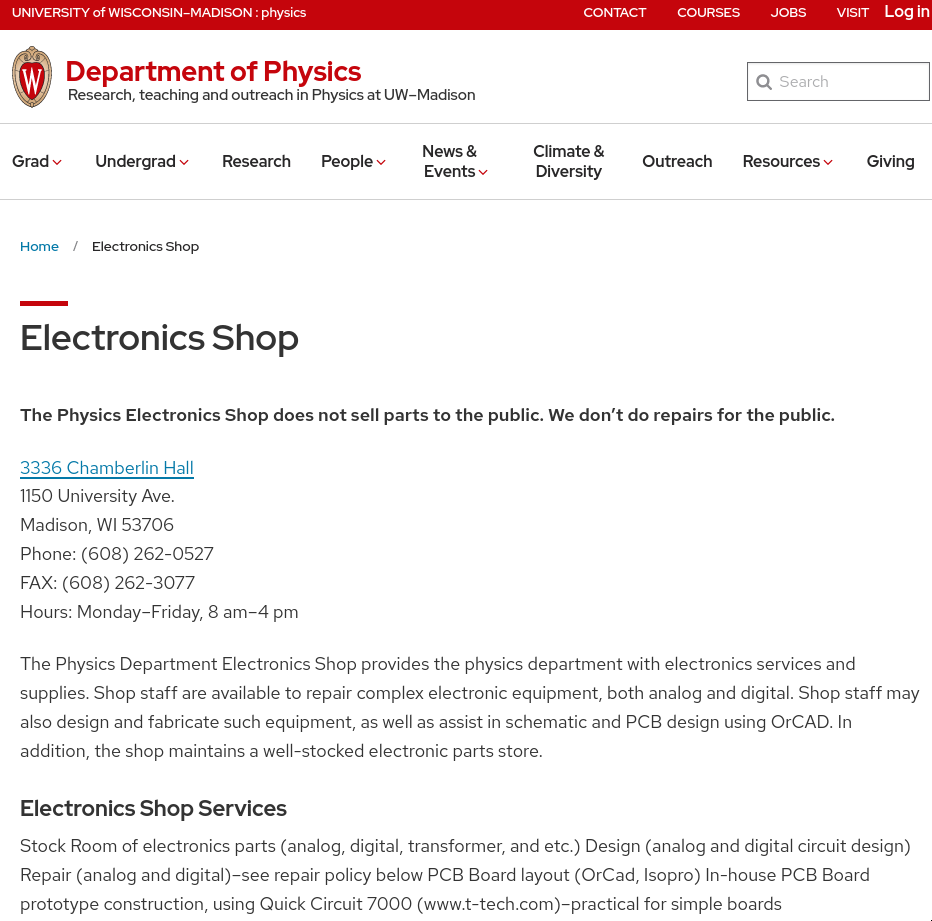
\includegraphics[width=\textwidth]{"./madison-physics.png"}
\end{frame}

\begin{frame}\frametitle{UW-Madison Physical Sciences Lab}
  
\includegraphics[width=\textwidth]{"./psl.png"}
\end{frame}

\begin{frame}\frametitle{Purdue Amy Facility}
  
\includegraphics[width=\textwidth]{"./amy.png"}
\end{frame}

\begin{frame}\frametitle{University of Washington}
  
\includegraphics[width=\textwidth]{"./washington.png"}
\end{frame}

\begin{frame}\frametitle{University of Colorado Boulder}
  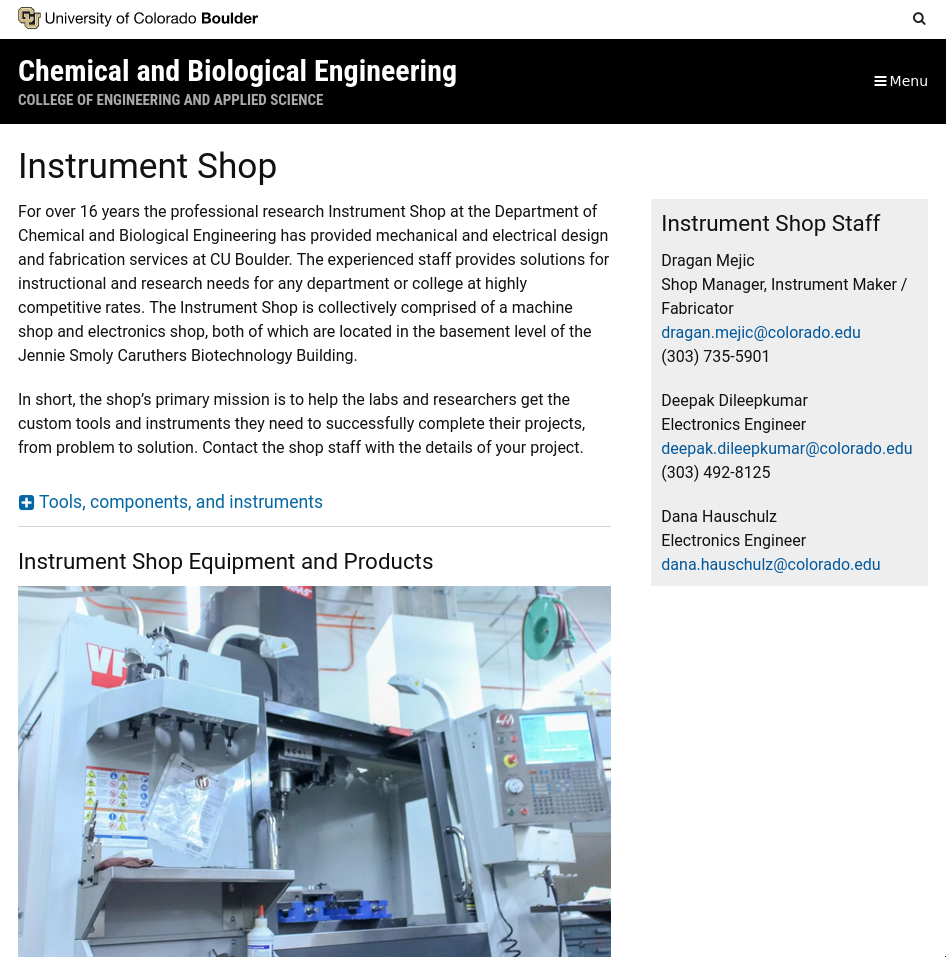
\includegraphics[width=\textwidth]{"./cu-boulder.png"}
\end{frame}

\begin{frame}\frametitle{University of Pittsburgh}
  
\includegraphics[width=\textwidth]{"./pittsburgh.png"}
\end{frame}

\begin{frame}\frametitle{Indiana University Bloomington}
  
\includegraphics[width=\textwidth]{"./bloom.png"}
\end{frame}

\begin{frame}\frametitle{UNC Chapel Hill}
  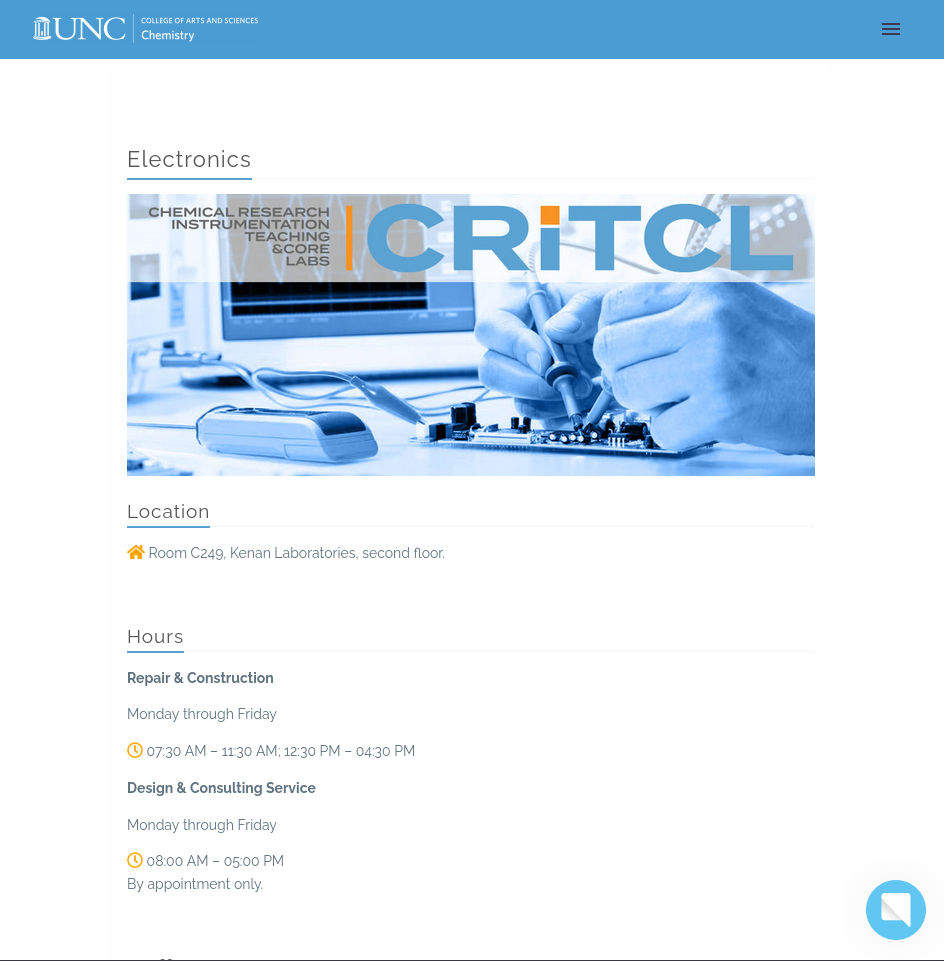
\includegraphics[width=\textwidth]{"./unc.png"}
\end{frame}

\begin{frame}\frametitle{Arizona State University}
  
\includegraphics[width=\textwidth]{"./asu.png"}
\end{frame}

\begin{frame}\frametitle{Stanford}
  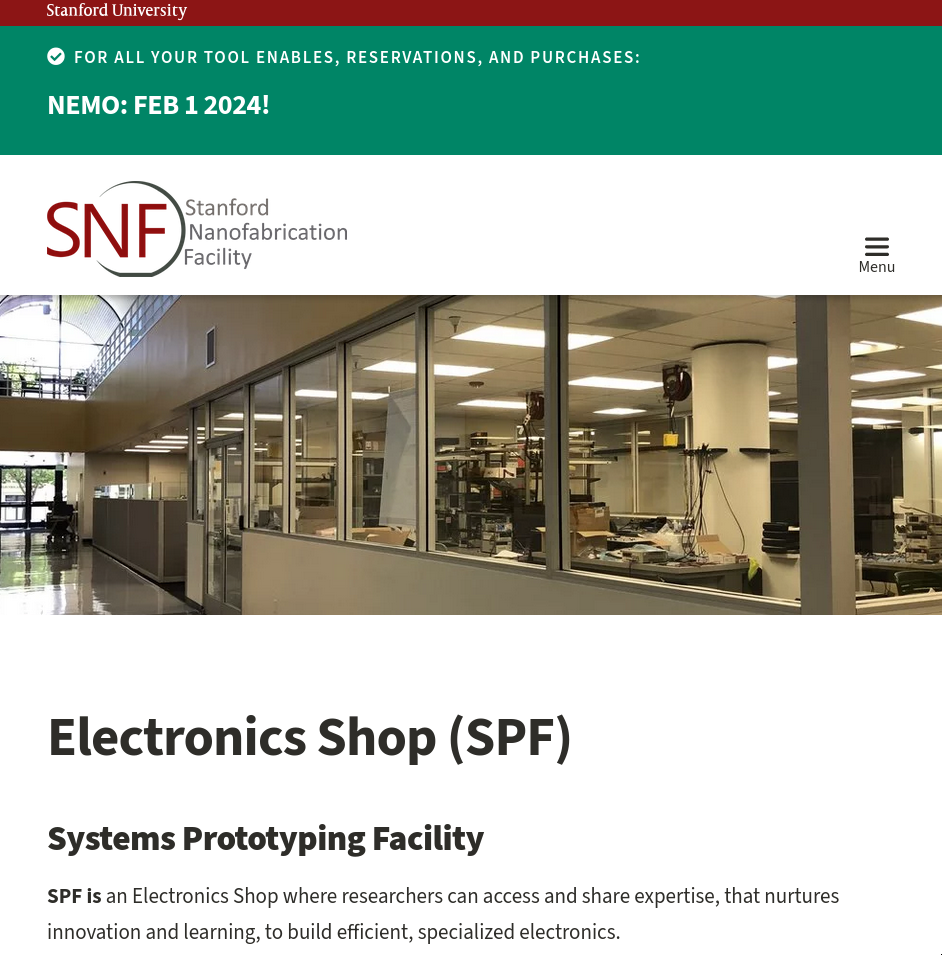
\includegraphics[width=\textwidth]{"./stanford.png"}
\end{frame}

\begin{frame}\frametitle{Brown}
  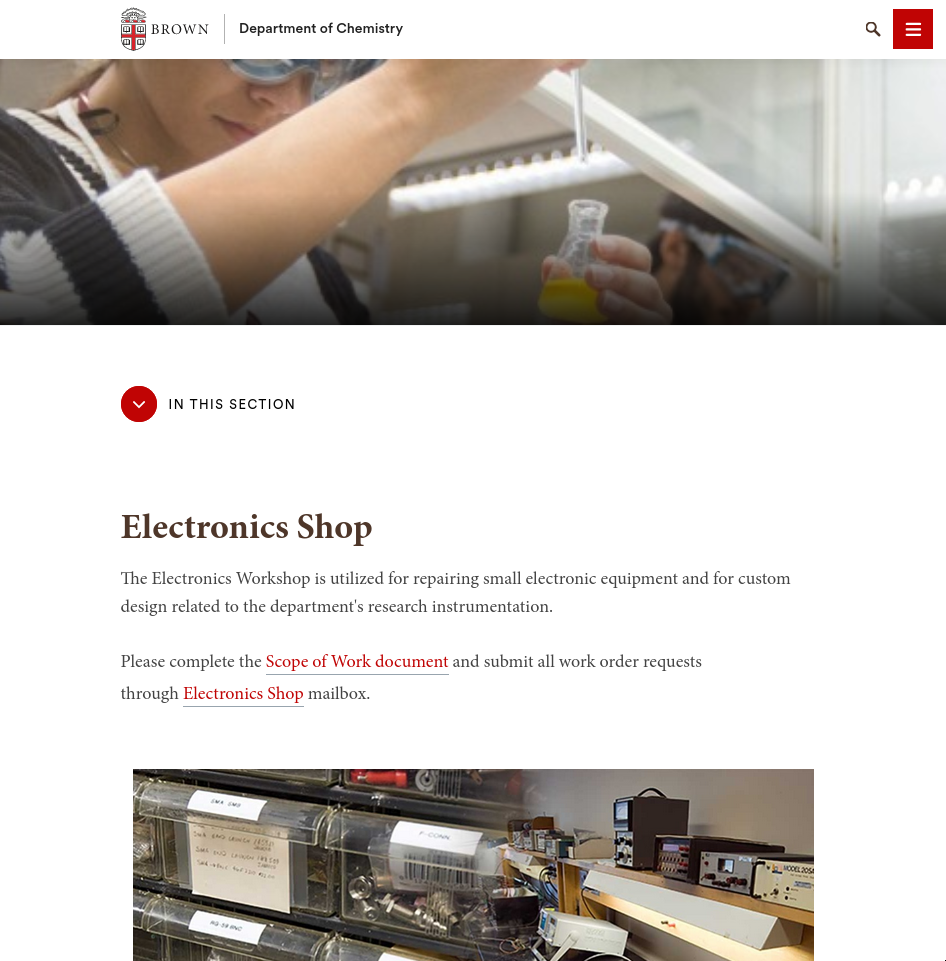
\includegraphics[width=\textwidth]{"./brown.png"}
\end{frame}

}

\section{Custom Research Electronics}

\begin{frame}
  \huge
  Custom electronics for research?
\end{frame}

\begin{frame}\frametitle{Electronics as Research}
  Electronics development has a key role to play in higher education \\
  \& cutting-edge research.
  \begin{itemize}
    \item lowered cost
    \item greater reproducibility
    \item automation, high throughput
    \item creativity and niche application
  \end{itemize}
\end{frame}

\begin{frame}\frametitle{XyloTron}
  \fbox{
    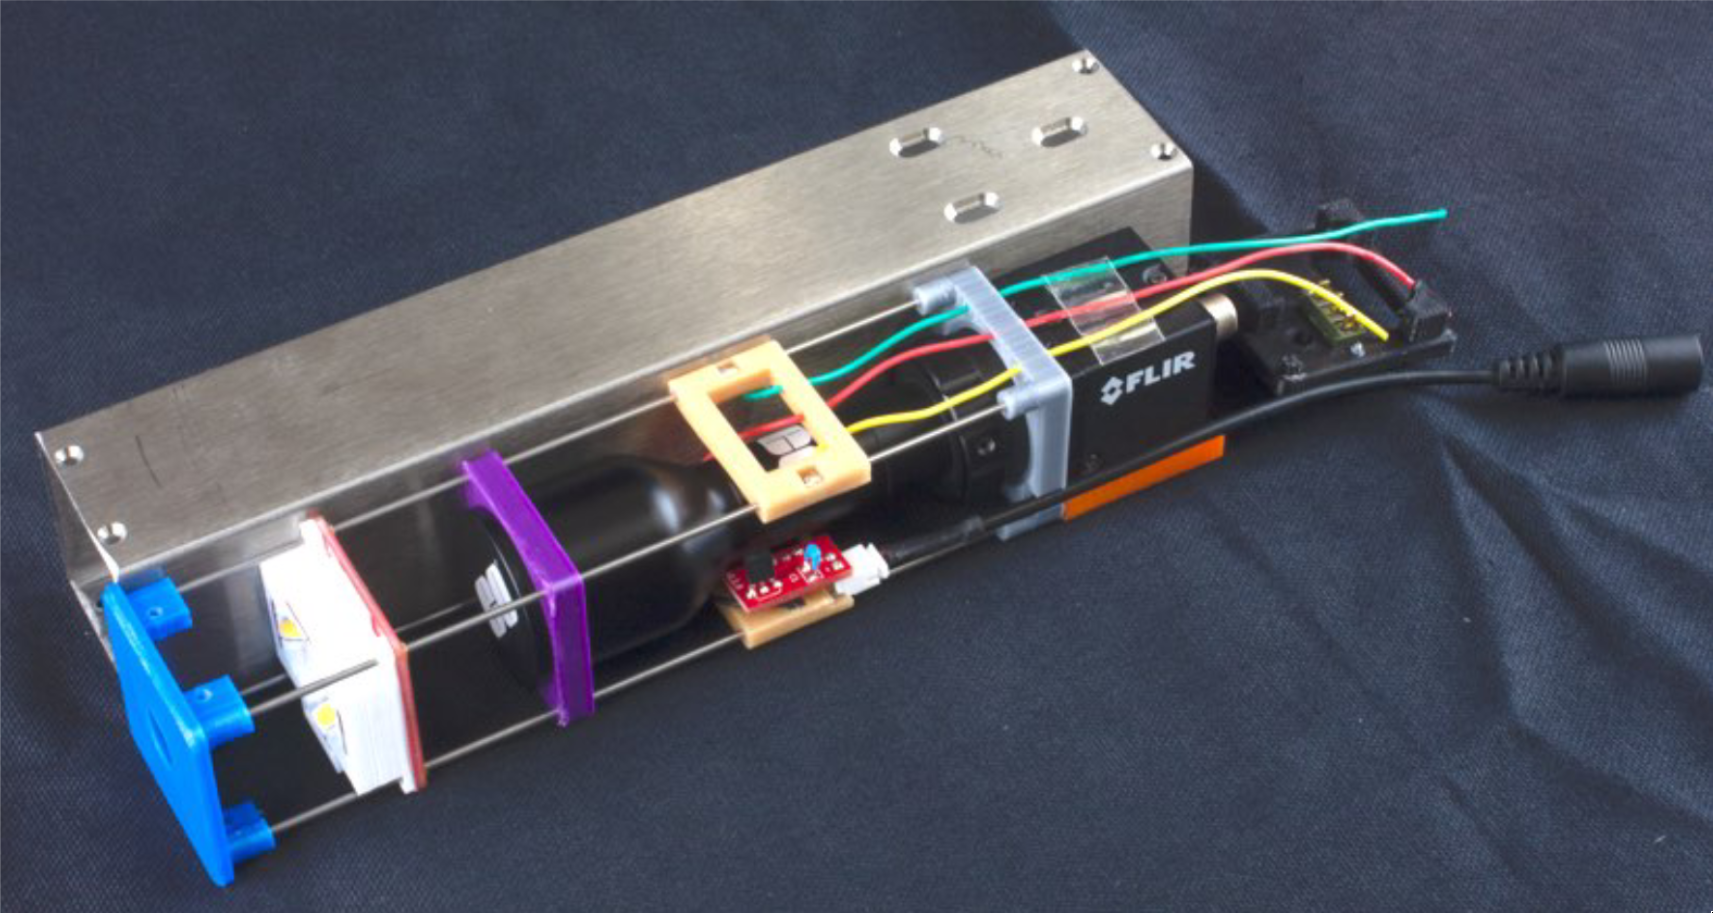
\includegraphics[width=\textwidth]{"./xylotron.pdf"}
  }
\end{frame}

\begin{frame}\frametitle{XyloTron}
  xylotron picture here please
\end{frame}

\begin{frame}\frametitle{Gas Uptake}
  \fbox{
    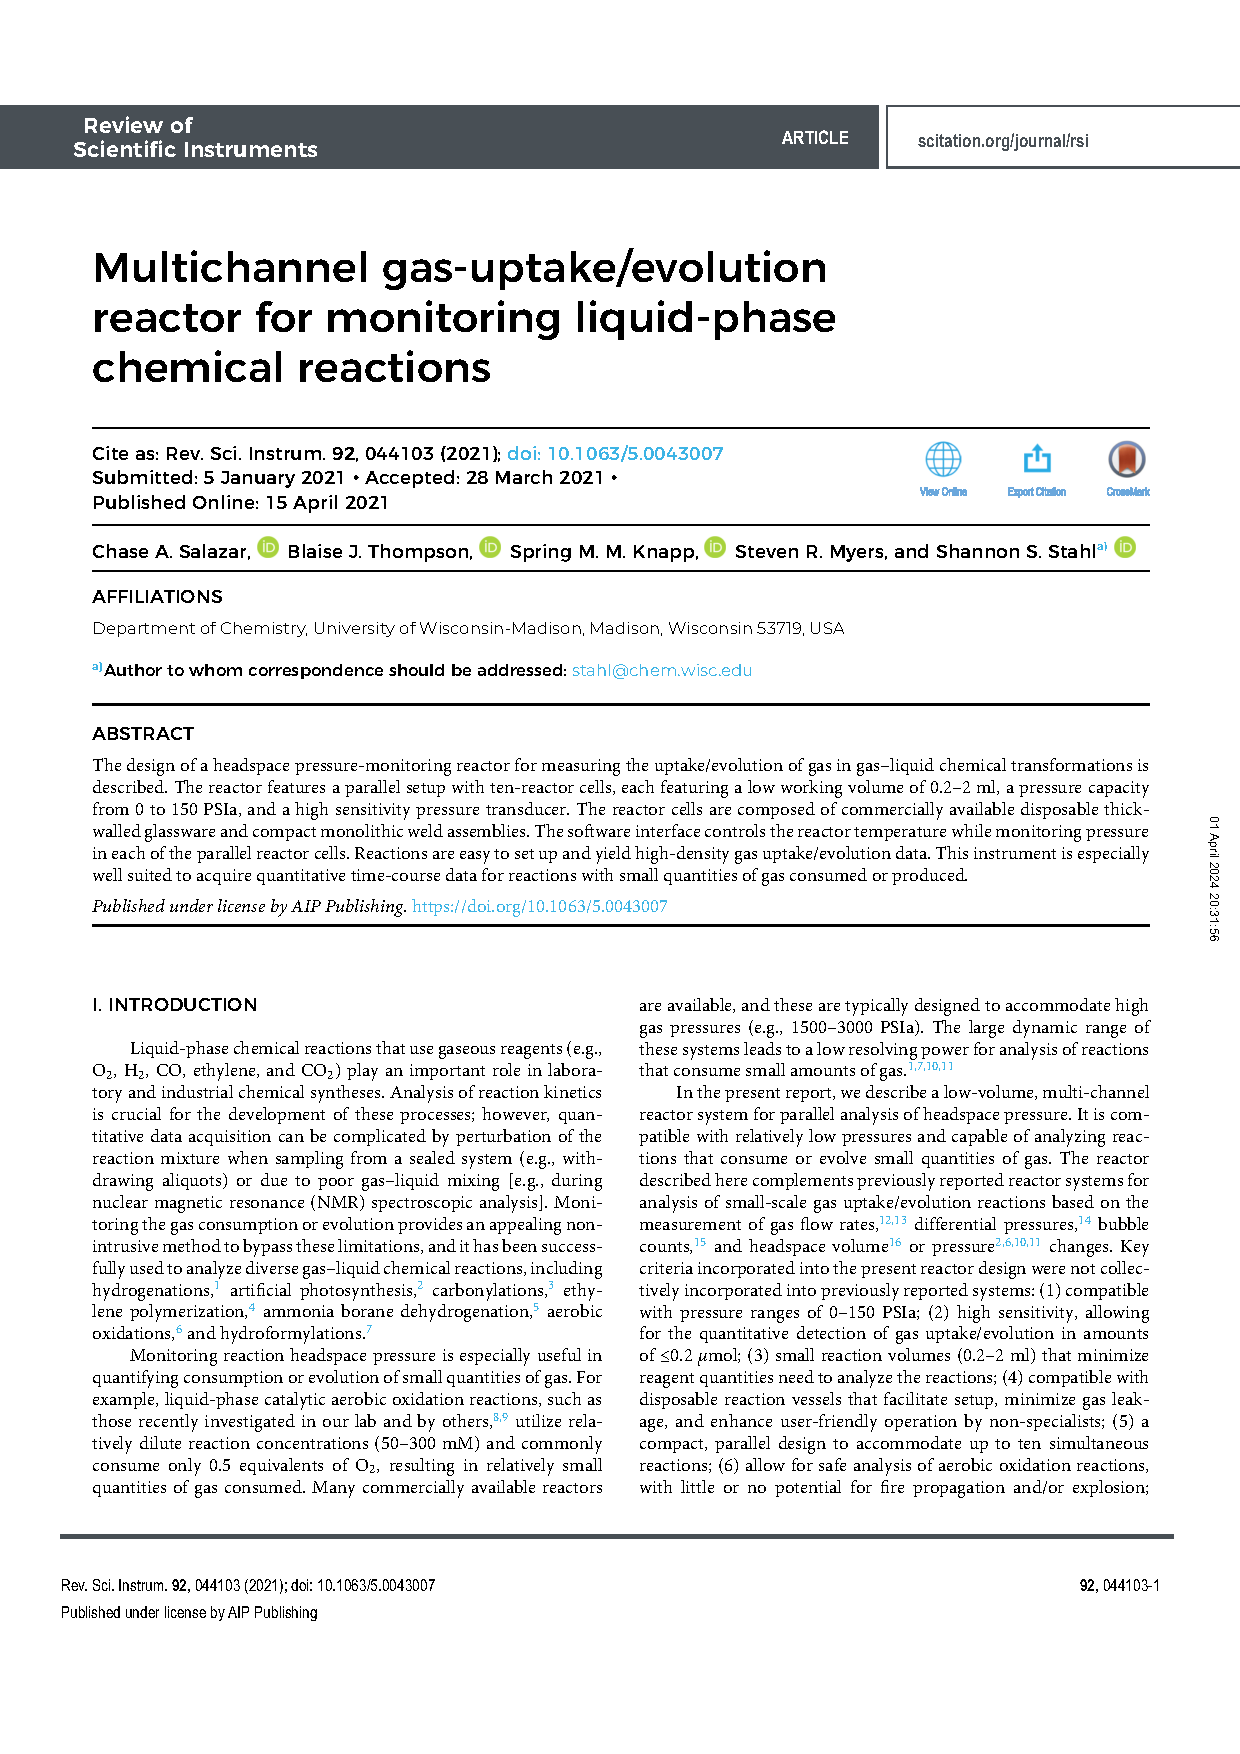
\includegraphics[width=\textwidth]{"./gas-uptake.pdf"}
  }
\end{frame}

\begin{frame}\frametitle{Gas Uptake}
  gas uptake picture here please
\end{frame}

\begin{frame}\frametitle{Photoreactor}
  \fbox{
    \includegraphics[width=\textwidth]{"./lampkin.pdf"}
  }
\end{frame}

\begin{frame}\frametitle{Photoreactor}
  photoreactor picture here please
\end{frame}


\begin{frame}\frametitle{Photoreactor}
  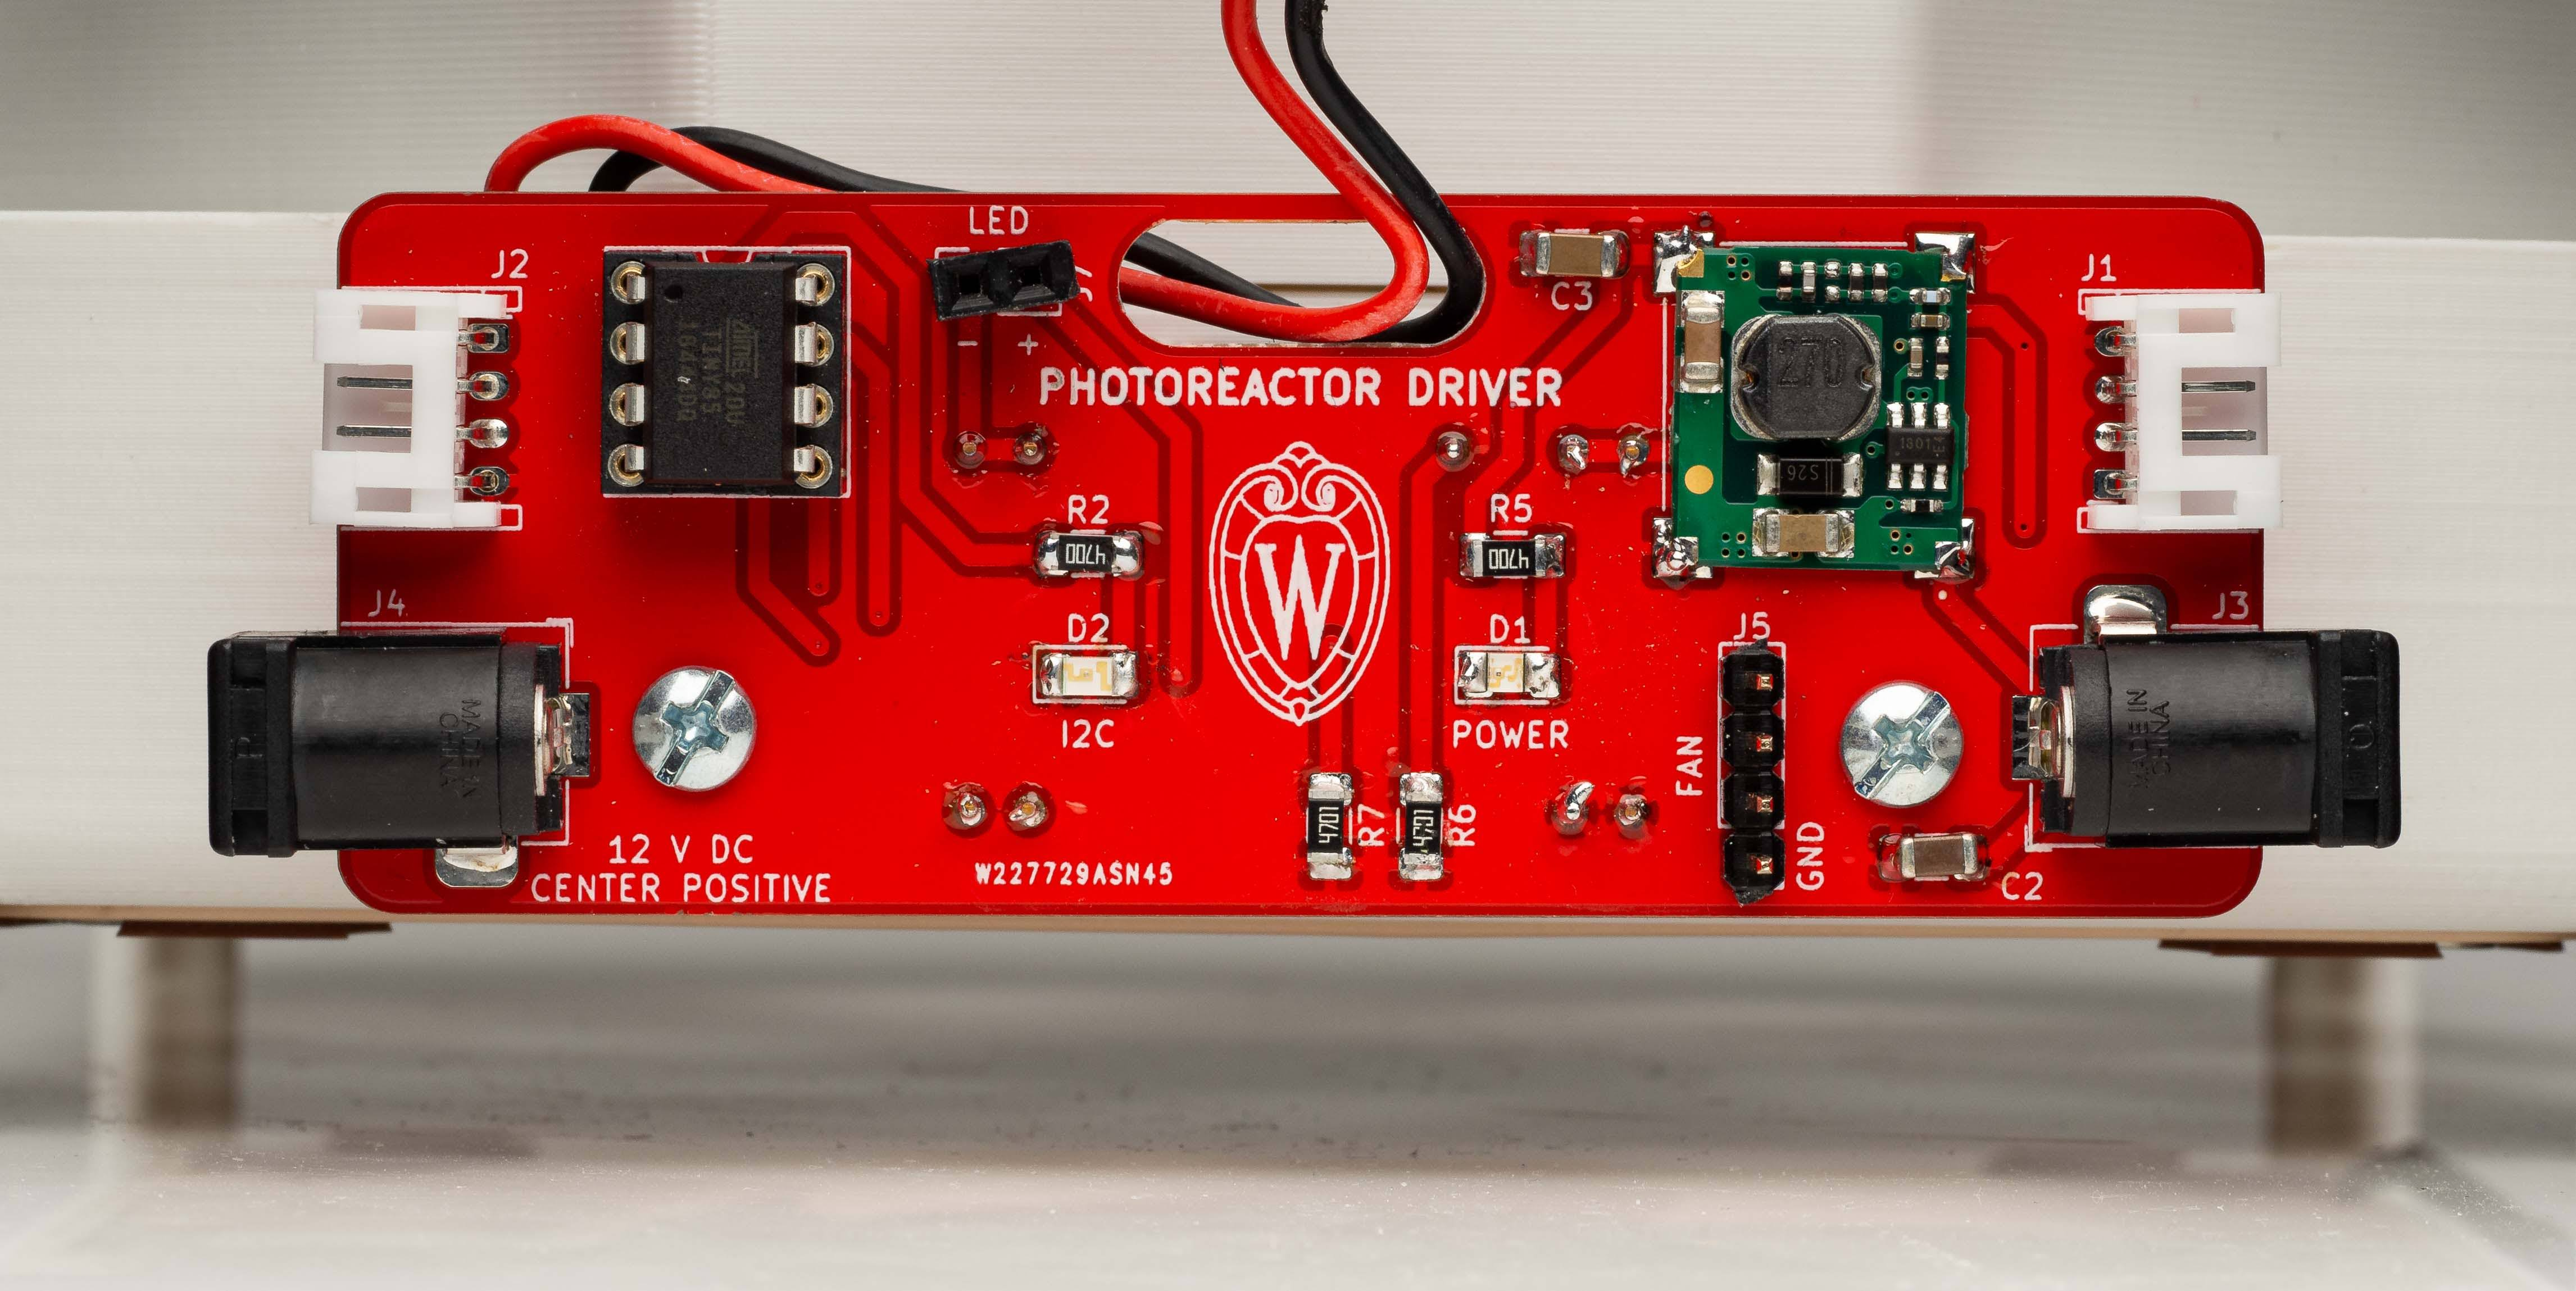
\includegraphics[width=\textwidth]{"./Philip (27).jpg"}
\end{frame}

\begin{frame}\frametitle{Oscillator}
  \fbox{
    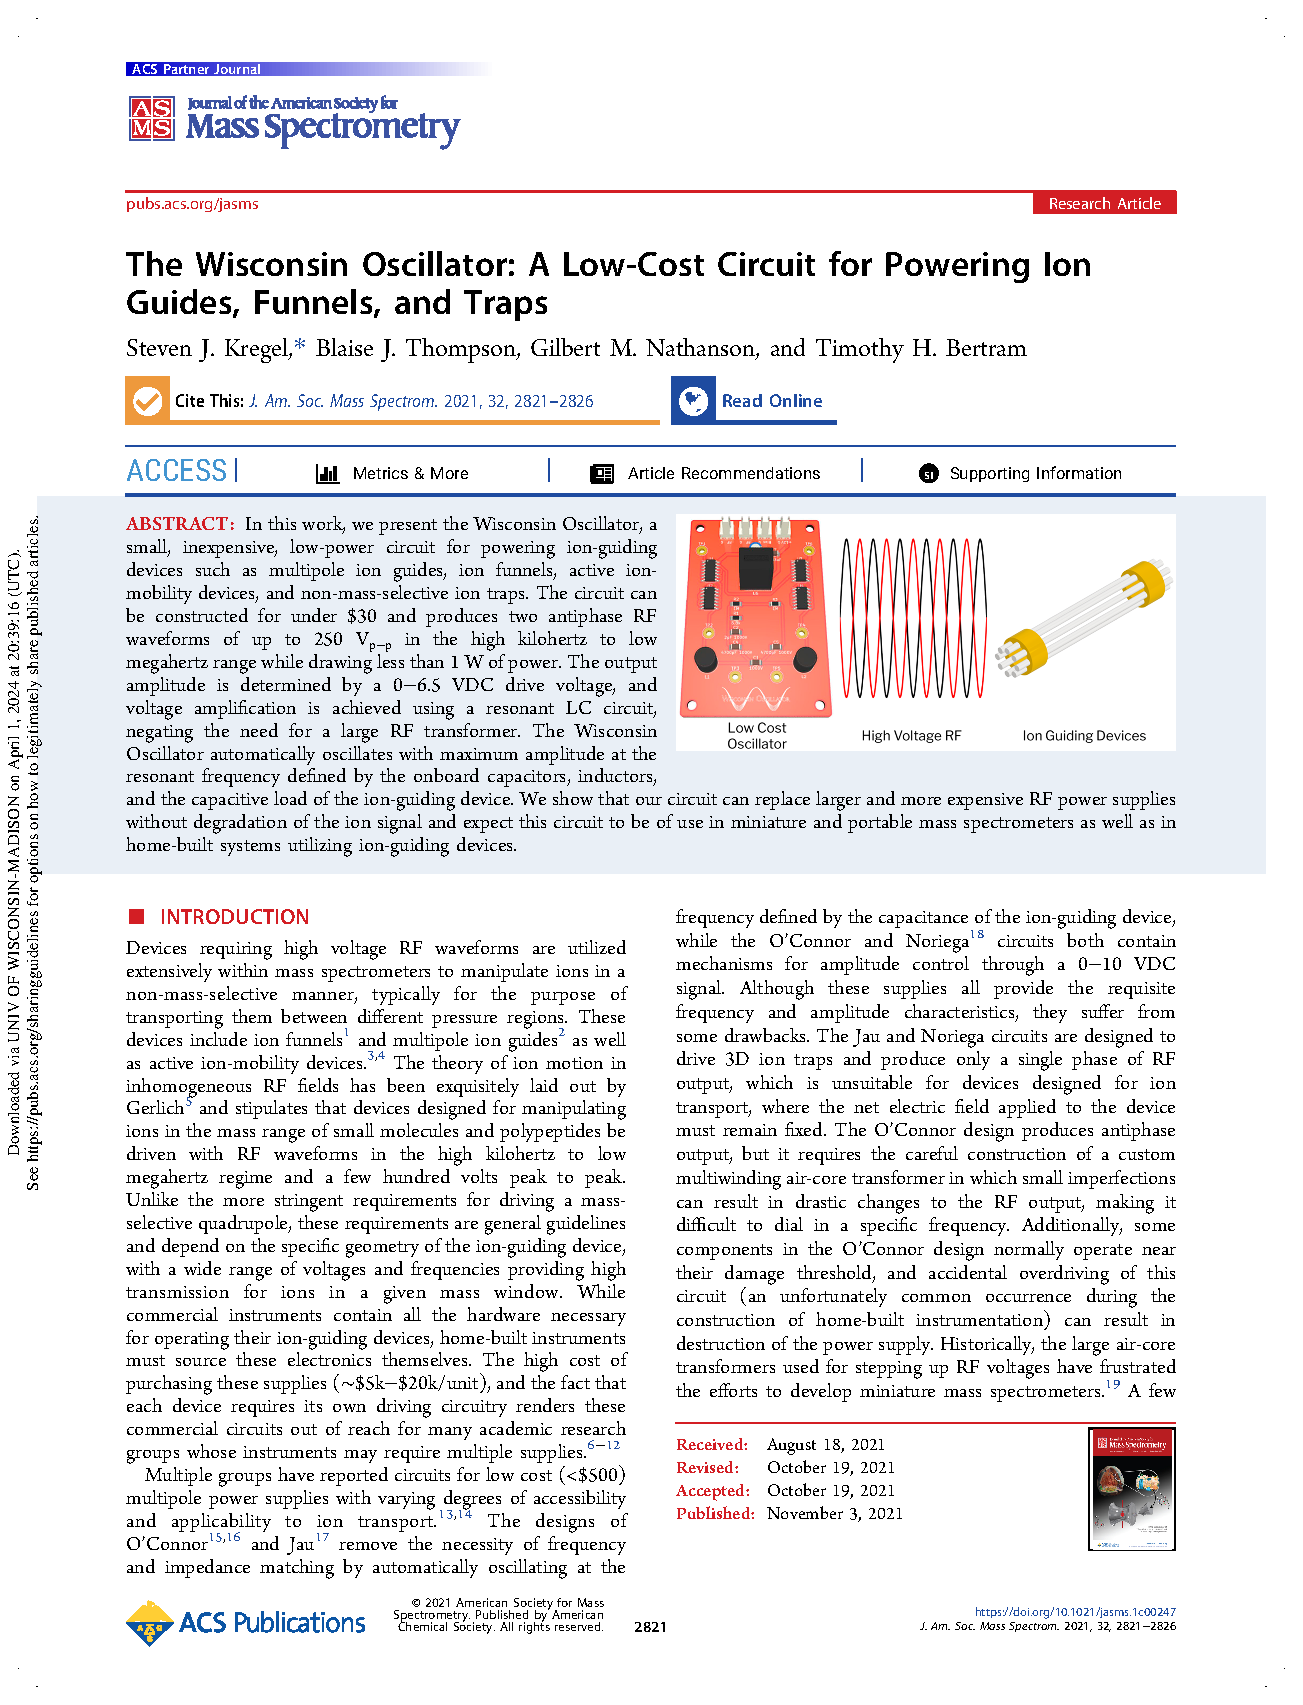
\includegraphics[width=\textwidth]{"./kregel.pdf"}
  }
\end{frame}

\begin{frame}\frametitle{Oscillator}
  oscillator picture here please
\end{frame}

\begin{frame}\frametitle{Teaching}
  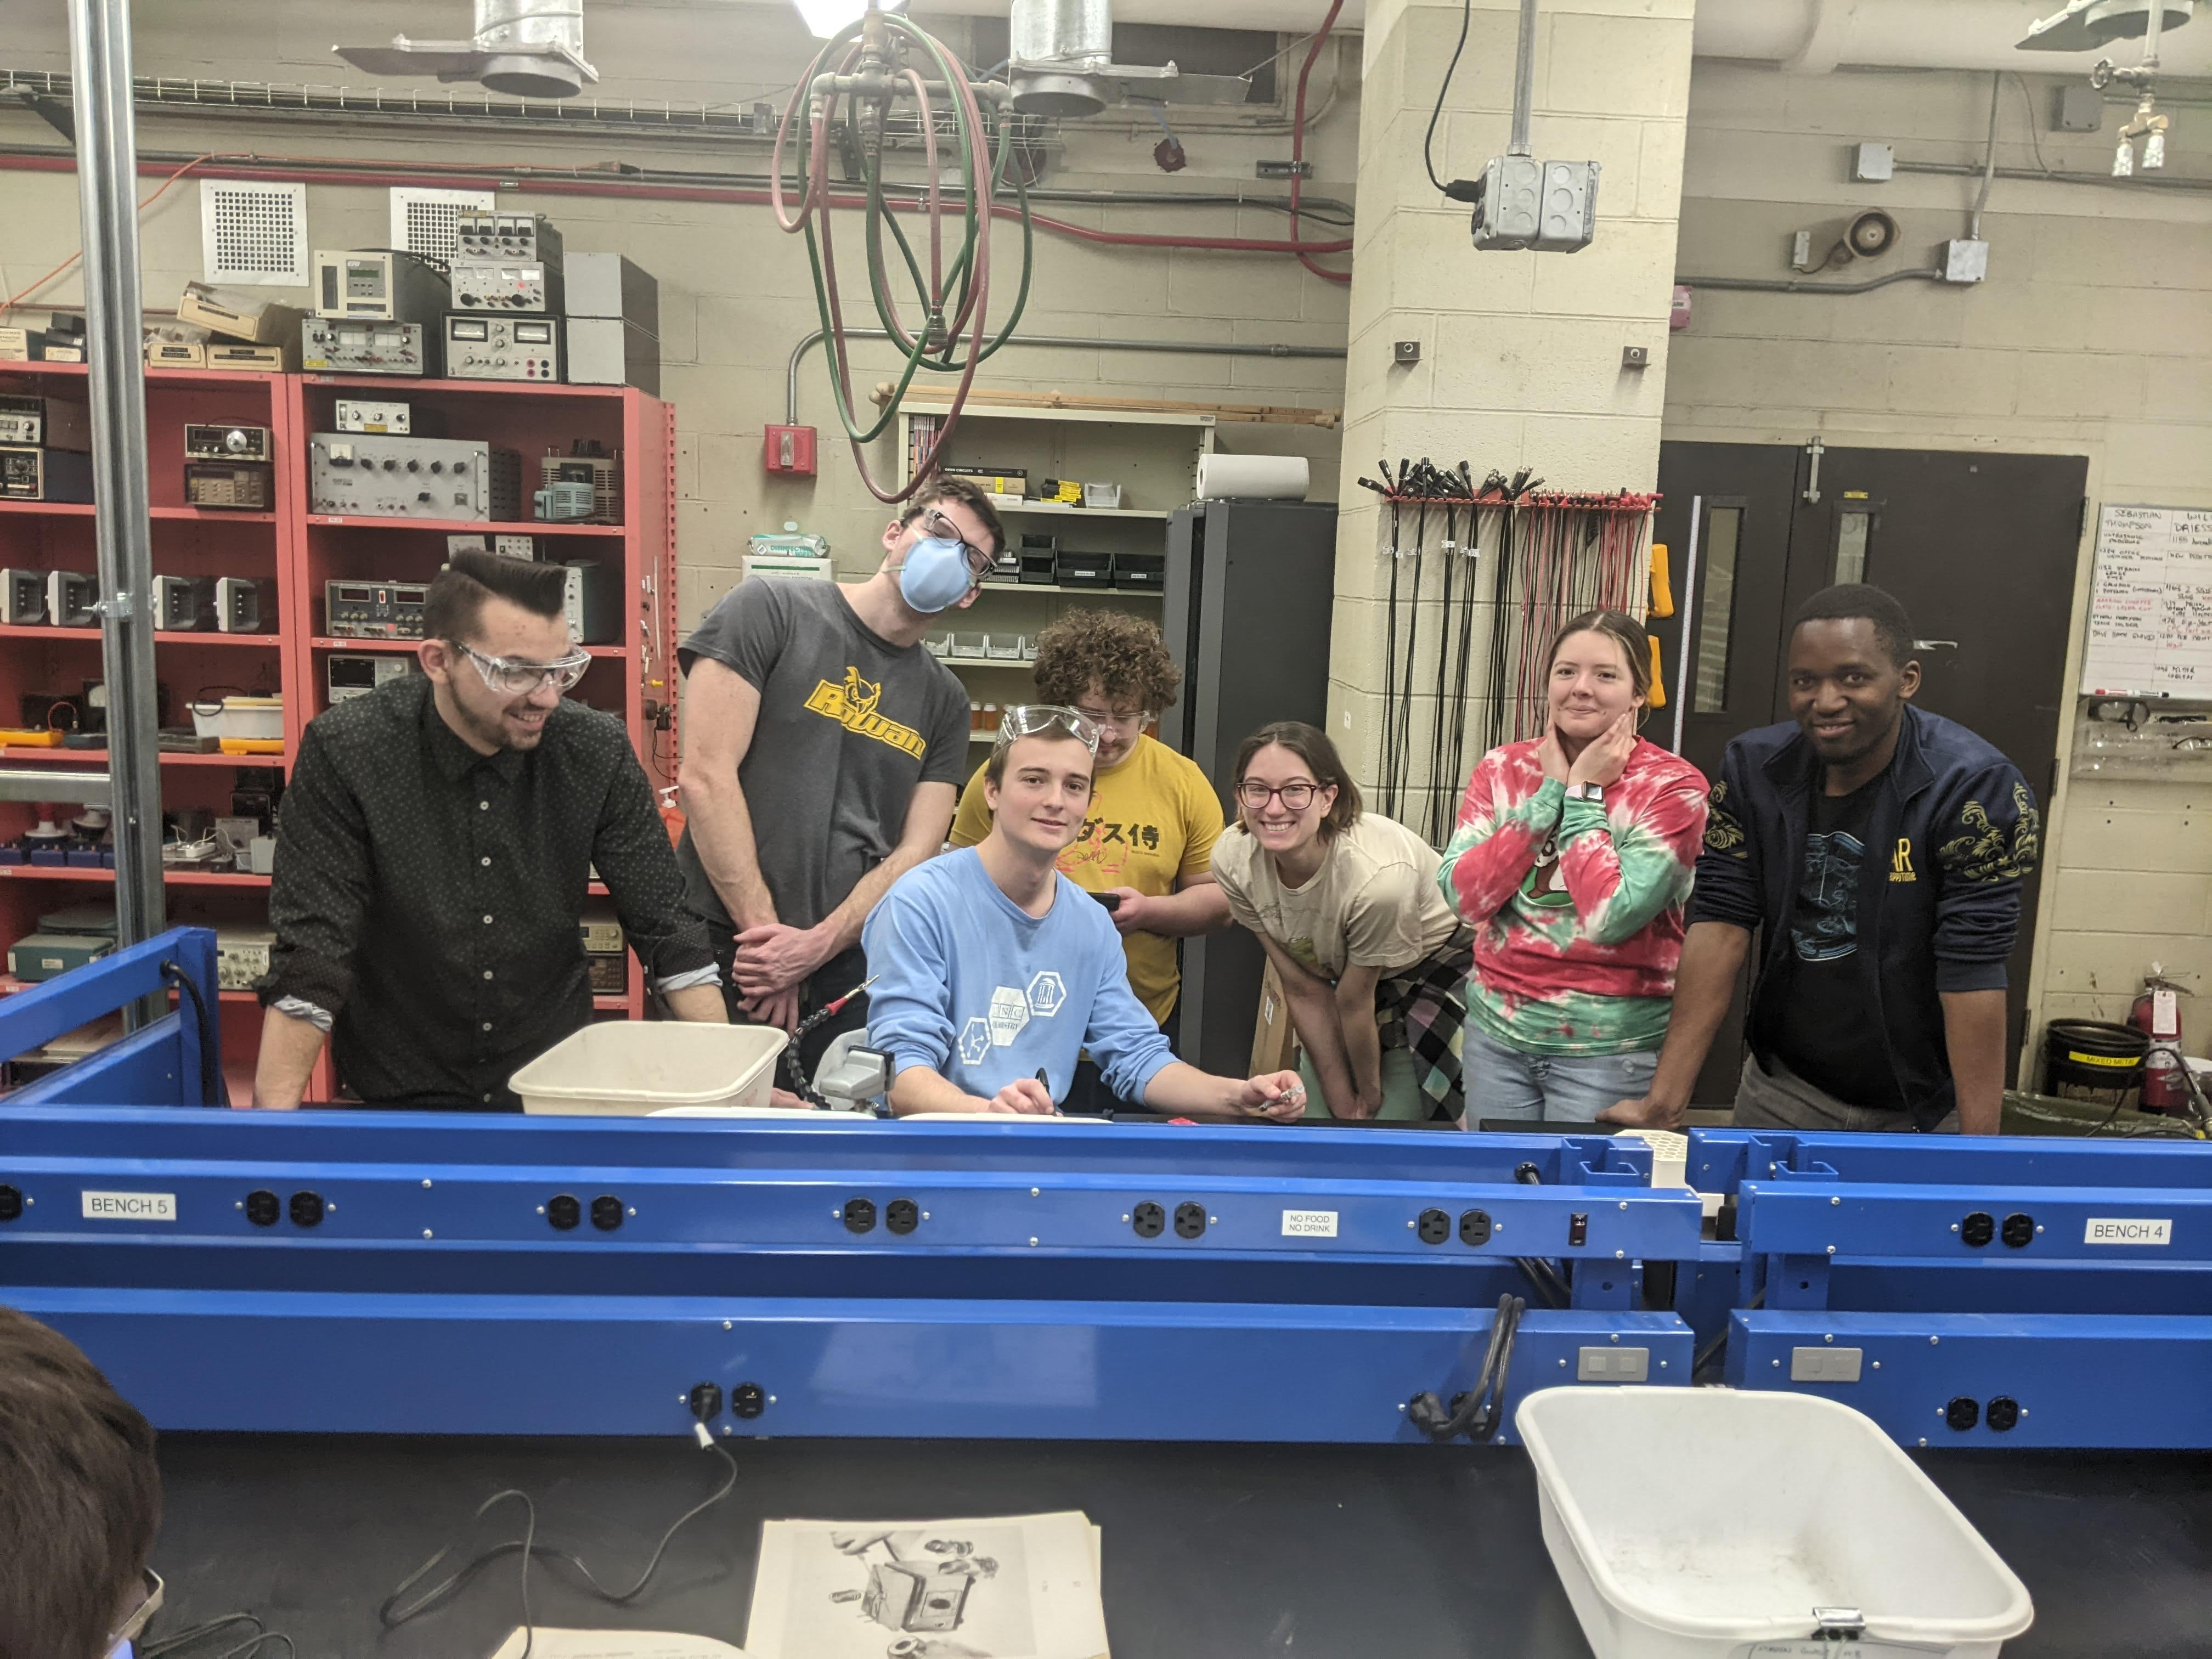
\includegraphics[width=\textwidth]{"./PXL_20230203_192355031.jpg"}
\end{frame}

\begin{frame}\frametitle{Workspace}
  workspace
\end{frame}

\begin{frame}\frametitle{Electronics: More Accessible than Ever}
  arduino
  rpi
  oshpark
  kicad
  adafruit, sparkfun
  kits
\end{frame}

\begin{frame}\frametitle{Open Source Hardware}
  \fbox{
    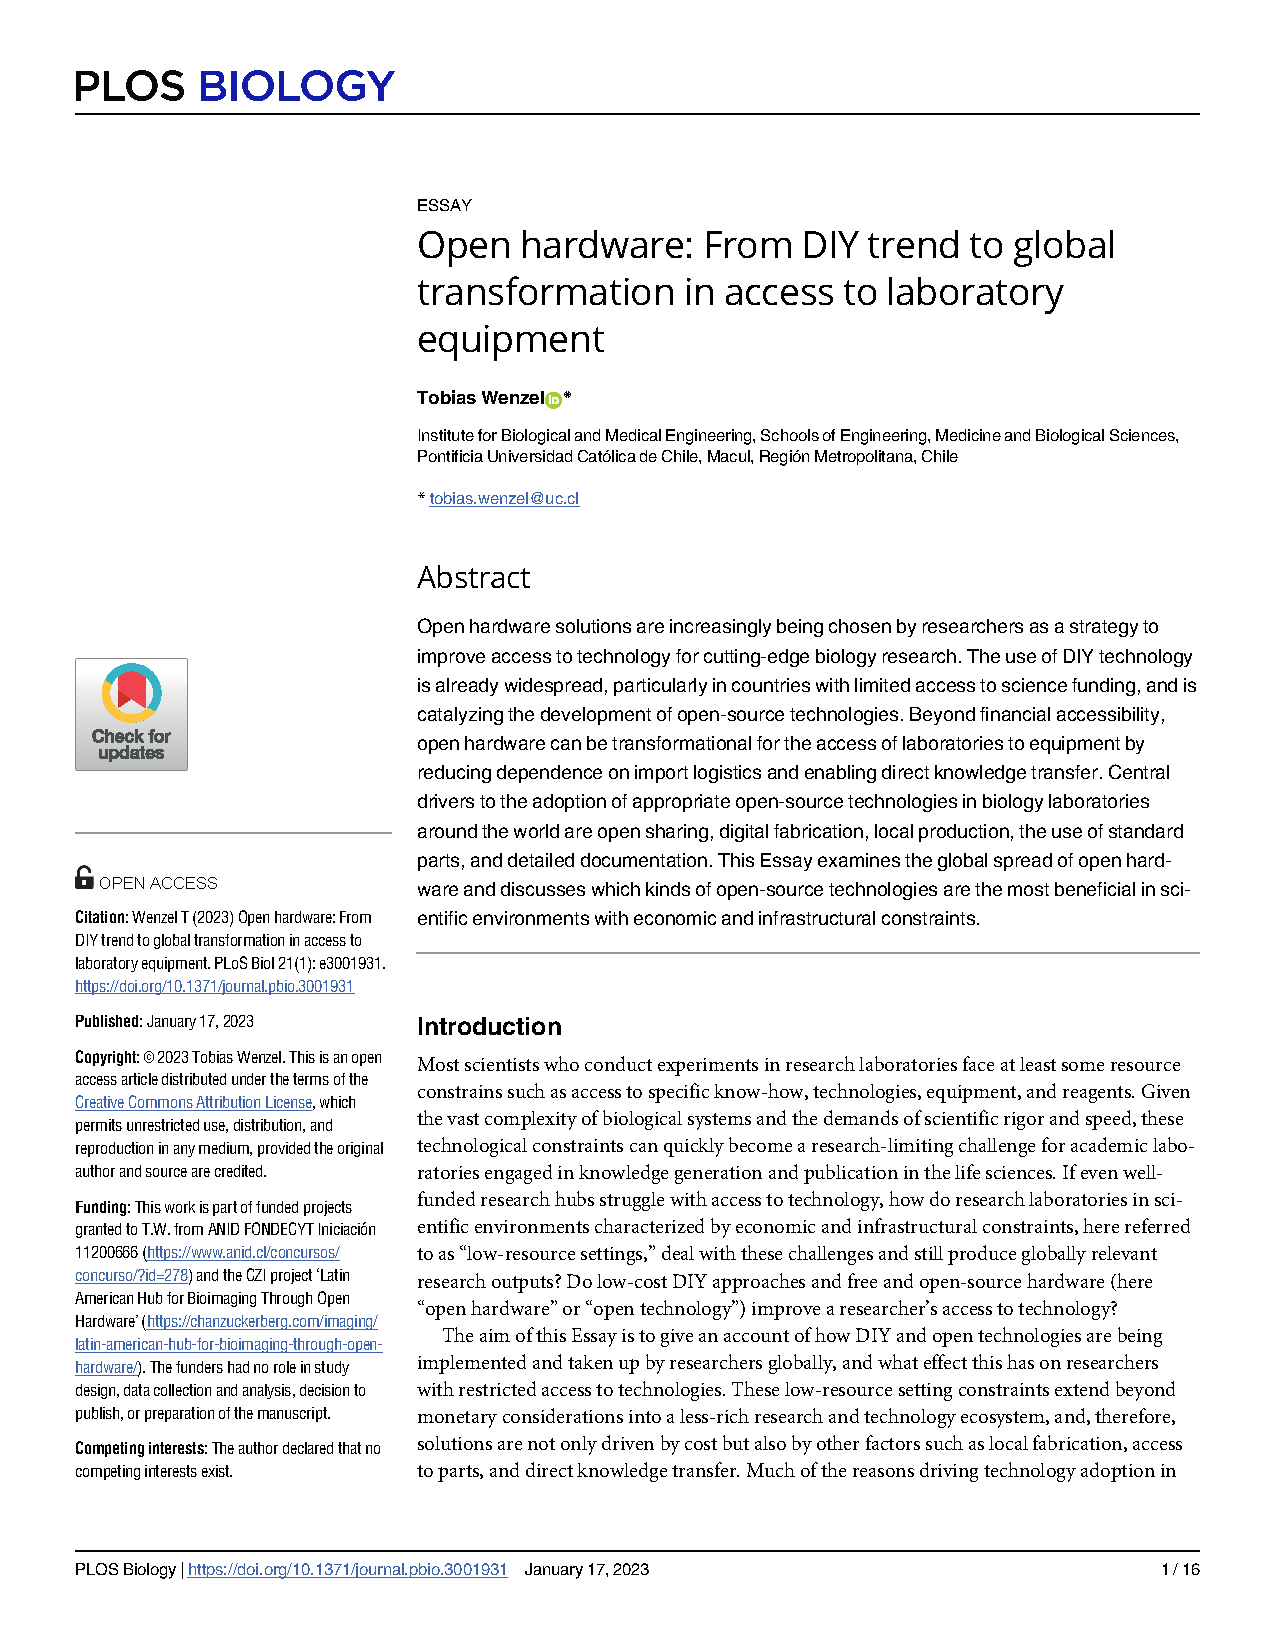
\includegraphics[width=\textwidth]{"./journal.pbio.3001931.pdf"}
  }
\end{frame}

\begin{frame}\frametitle{Open Source Hardware}
  \centering
  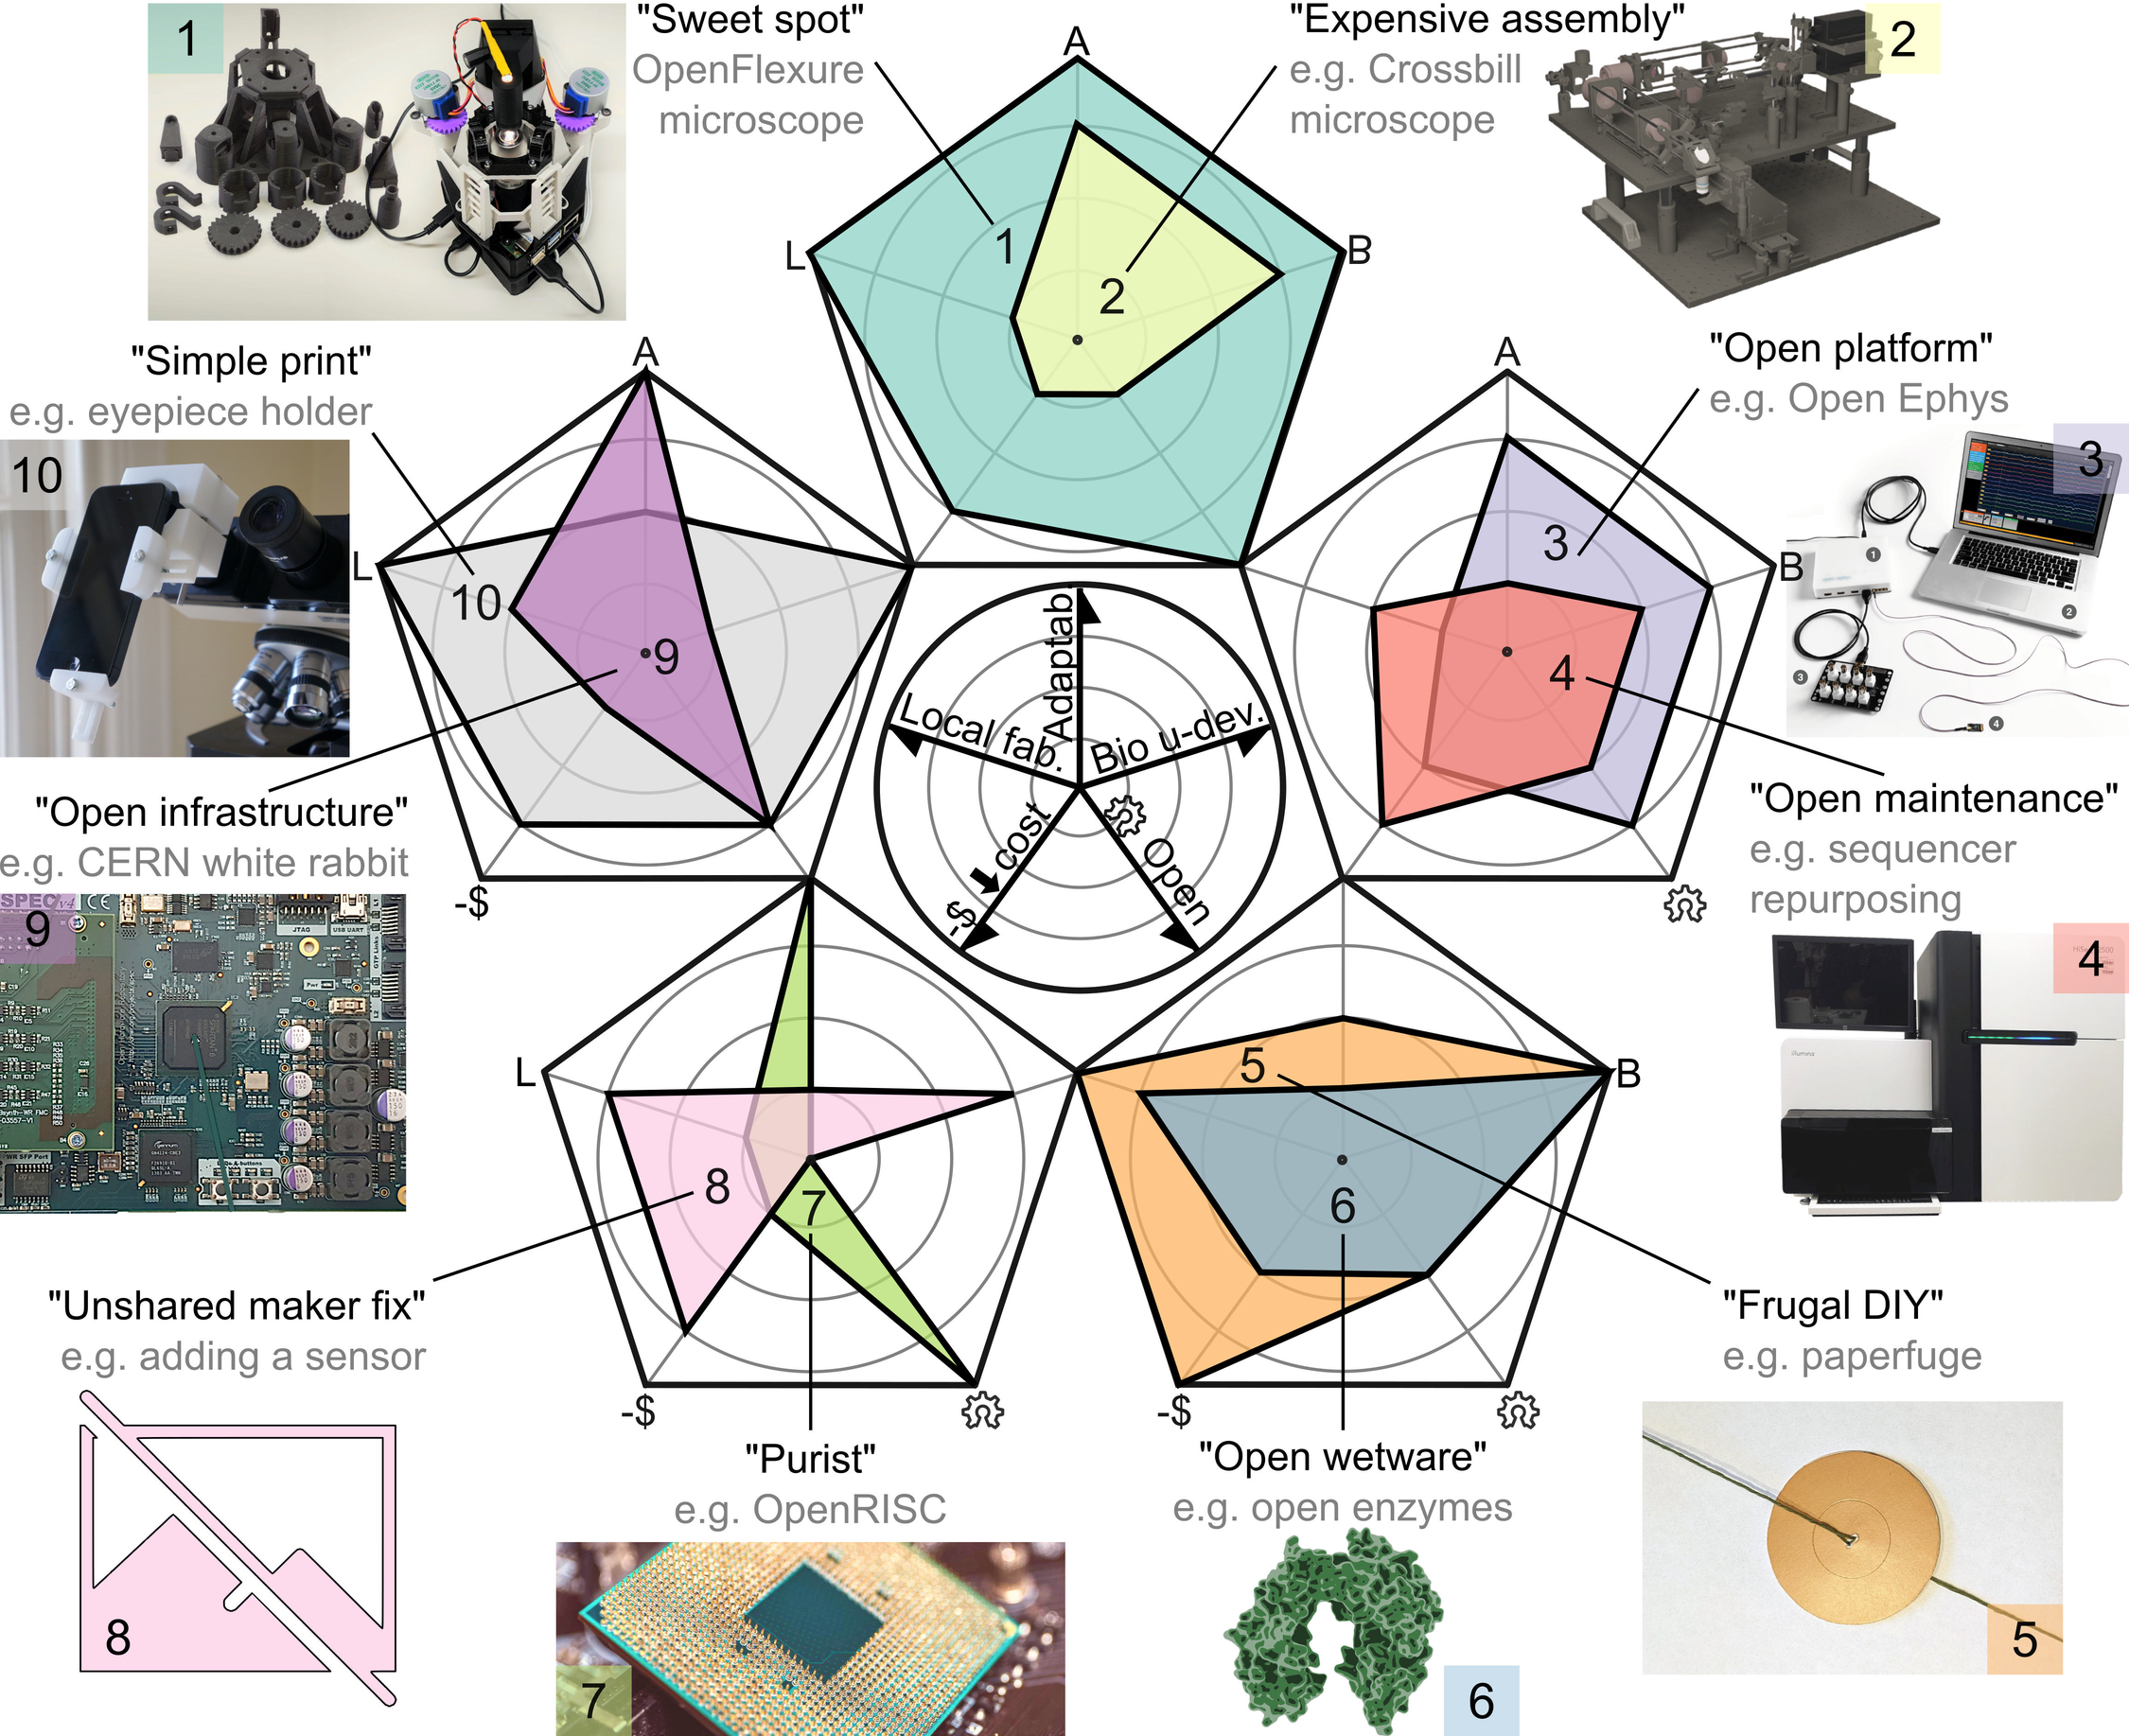
\includegraphics[width=3.5in]{"./journal.pbio.3001931.g002.PNG"}
\end{frame}

\section{Appliance Maintenance}

\begin{frame}
  \huge
  Repair and maintenance of research equipment.
\end{frame}

\begin{frame}\frametitle{Amber Bartz}
  \begin{columns}
    \begin{column}{0.33\textwidth}
      \includegraphics[width=\textwidth]{"./bartz.png"}
    \end{column}
    \begin{column}{0.67\textwidth}
      Amber Bartz \\
      Chemistry Electronics Shop \\
      afbartz@wisc.edu
      \vskip 3 em
      Check out Amber's poster presentation: \\
      \emph{What Researchers Should Know When Powering Lab Equipment}
    \end{column}
  \end{columns}
\end{frame}

\section{Safety}

\begin{frame}
  Electrical Safety \\
  as Viewed from the Shop
\end{frame}

\begin{frame}\frametitle{Safety}
  Researchers utilize advanced electronics. \\
  Researchers design and build custom instruments. \\
  Researchers rely on in-house repair. \\
  \vfill{}
  Let's think about safety implications!
\end{frame}

\begin{frame}\frametitle{Humility}
  I'm not a safety expert... talking at CSHEMA is a bit intimidating.
  \vfill
  I'm glad you are dedicating a symposium to electrical safety.
  \vfill
  I have no idea how to think about certification...
  \vfill
  I hope we can work together.
\end{frame}

\begin{frame}\frametitle{Safety}
  Cutting-edge researchers will inevitably customize/create electronic circuits.
  \vfill
  Hopefully, the electronics shop can be a place to do this work under professional supervision!
  \vfill
  We don't have the time or the staff to look over every shoulder...
  ...instead, we try to convince researchers that they have a professional responsibility to care about electrical safety.
\end{frame}

\begin{frame}\frametitle{Safety}
  Two categories of electrical hazard:
  \begin{itemize}
    \item electrocution
    \item fire
  \end{itemize}
\end{frame}

\subsection{Electrocution}

\begin{frame}{Electrocution}
  \begin{snugshade}
    Electrical hazards represent a serious, widespread occupational danger; practically all members of the workforce are exposed to electrical energy during the performance of their daily duties, and electrocutions occur to workers in various job categories.
    Many workers are \hl{unaware} of the potential electrical hazards present in their work environment, which makes them more vulnerable to the danger of electrocution.
  \end{snugshade}
  \vfill
  \tiny
  WORKER DEATHS BY ELECTROCUTION \\
  A Summary of NIOSH Surveillance and Investigative Findings \\
  May 1998
\end{frame}


\begin{frame}{Current Kills}
  Relatively small amounts of current can be very dangerous!
  \begin{itemize}
    \item 1 mA - barely perceptible
    \item 16 mA - maximum current an average person can grasp and ``let go''
    \item 20 mA - paralysis of respiratory muscles
    \item 100 mA - ventricular fibrillation threshold
    \item 2000 mA - cardiac standstill and internal organ damage
    \item 15000 mA - fuse / breaker opens circuit
  \end{itemize}
  A typical LED draws 20 mA. \\
  Fuses and breakers will NOT protect you from death by electrocution!
  \vfill
  \tiny
  WORKER DEATHS BY ELECTROCUTION \\
  A Summary of NIOSH Surveillance and Investigative Findings \\
  May 1998
\end{frame}

\begin{frame}{Current and Voltage}
  \begin{columns}
    \begin{column}{0.33\textwidth}
      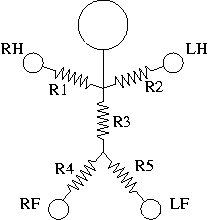
\includegraphics[width=\textwidth]{"./resistor-person.png"}
    \end{column}
    \begin{column}{0.67\textwidth}
      Current and voltage are related by Ohm's Law.
      \begin{equation*}
        V = IR
      \end{equation*}
      Larger voltages drive more current through your body.
    \end{column}
  \end{columns}
\end{frame}

\begin{frame}{Current and Voltage}
  \begin{columns}
    \begin{column}{0.33\textwidth}
      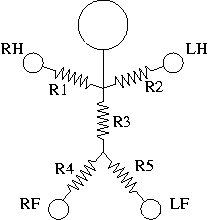
\includegraphics[width=\textwidth]{"./resistor-person.png"}
    \end{column}
    \begin{column}{0.67\textwidth}
      ``Typical'' resistance across the human body: \\ as low as $10\mathrm{k}\Omega$.
      Solve for voltage driving 10 mA
      \begin{eqnarray*}
        V &=& 10 \mathrm{mA} \times 10 \mathrm{k}\Omega \\
        V &=& 100 \mathrm{V}
      \end{eqnarray*}
      Every device plugged into the wall is at least \hl{120V}.
    \end{column}
  \end{columns}
\end{frame}

\begin{frame}{Wet and Dry}
  \begin{columns}
    \begin{column}{0.33\textwidth}
      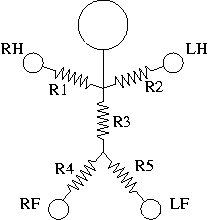
\includegraphics[width=\textwidth]{"./resistor-person.png"}
    \end{column}
    \begin{column}{0.67\textwidth}
      Most resistance is at the skin.
      \vskip 2 em
      Resistance \hl{decreases} significantly if your skin is \hl{wet}.
    \end{column}
  \end{columns}
\end{frame}

\begin{frame}
  \frametitle{Typical Voltages}
  Treat anything above 30 V as an electrocution hazard.
  \begin{itemize}
    \item 5 V - USB power supply
    \item 120 V - typical lab appliance
    \item 120 V - typical vacuum roughing pump
    \item 1000 V - piezoelectric actuators
    \item 1000 V - photomultipliler tubes
    \item 3000 V - electron / ion multipliers
    \item 15000 V - X-Ray sources
    \item TODO: GEL ELECTROPHORESIS
  \end{itemize}
\end{frame}

\begin{frame}{Typical Voltages}
  \begin{columns}
    \begin{column}{0.33\textwidth}
      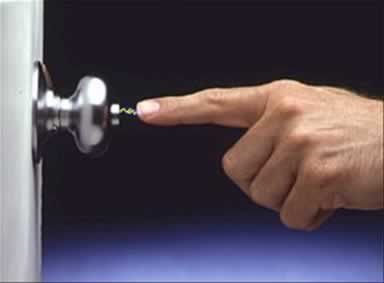
\includegraphics[width=\textwidth]{"./doorknob.png"}
      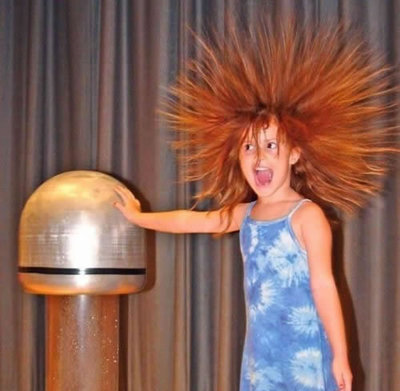
\includegraphics[width=\textwidth]{"./hair.png"}
    \end{column}
    \begin{column}{0.67\textwidth}
        Voltage is not necessarily dangerous,
        \vskip 2 em
        Know the current rating!
    \end{column}
  \end{columns}
\end{frame}

\begin{frame}{GFCI}
  \begin{columns}
    \begin{column}{0.33\textwidth}
      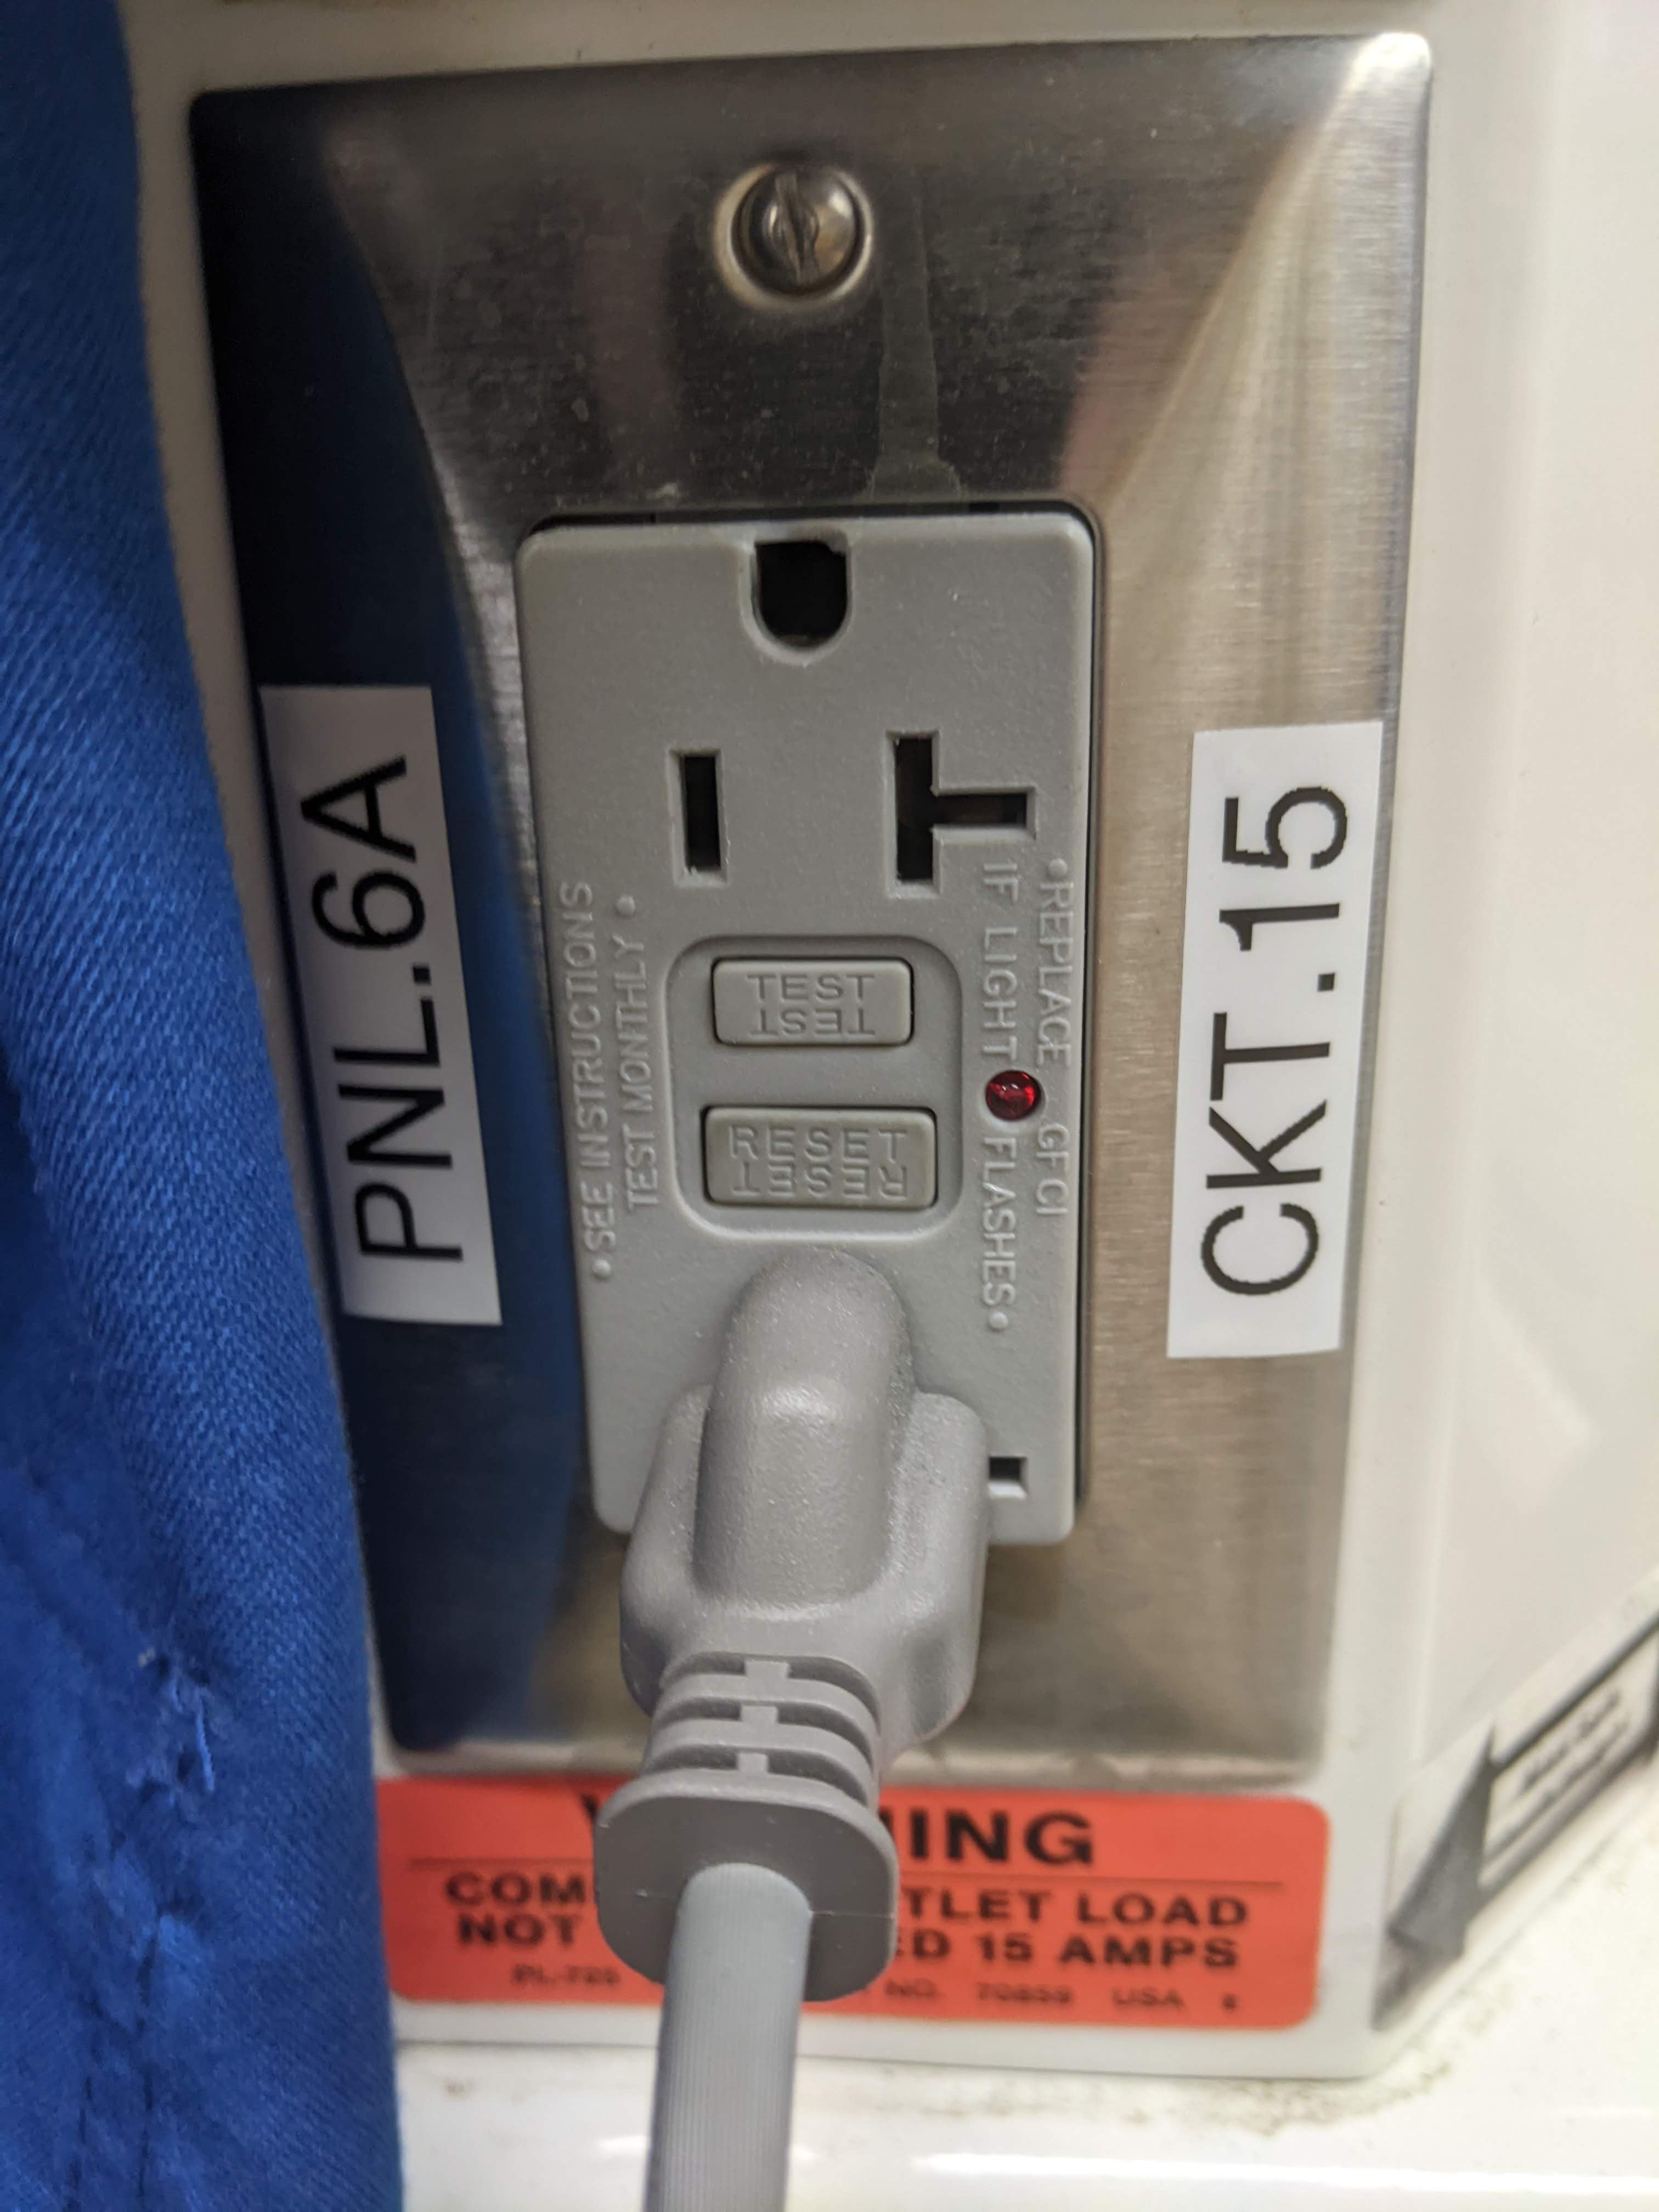
\includegraphics[width=\textwidth]{"./PXL_20230117_221804507.jpg"}
    \end{column}
    \begin{column}{0.67\textwidth}
      Designed specifically for shock protection.
      \vskip 2 em
      Ensure that no current is leaking out of circuit. \\
      Sensitive to a few mA.
      \vskip 2 em
      Will trip if used with large inductive loads (motors).
      \vskip 2 em
      Prone to weaken over time---replaced every ten years.
    \end{column}
  \end{columns}
\end{frame}

\begin{frame}{Recommendations for Avoiding Shock}
  Avoid contact with energized electrical circuits.
  \begin{itemize}
    \item NEVER work behind the outlet or in the walls.
    \item If it is safe to do so, work with only one hand. This precaution reduces the likelihood of accidents that result in current passing through the chest cavity.
    \item When it is necessary to handle equipment that is plugged in, be sure hands are dry and, when possible, wear nonconductive gloves and shoes with insulated soles.
    \item If an individual comes in contact with a live electrical conductor, do not touch the equipment, cord or person. Disconnect the power source from the circuit breaker or pull out the plug using a leather belt.
  \end{itemize}
\end{frame}

\begin{frame}{Recommendations for Avoiding Shock}
  Avoid mixing water and electricity.
  \begin{itemize}
    \item Minimize the use of electrical equipment in cold rooms or other areas where condensation is likely. If equipment must be used in such areas, mount the equipment on a wall or vertical panel.
    \item If water or a chemical is spilled onto equipment, shut off power at the main switch or circuit breaker and unplug the equipment.
  \end{itemize}
\end{frame}

\begin{frame}{Electrocution Hazard}
  \centering
  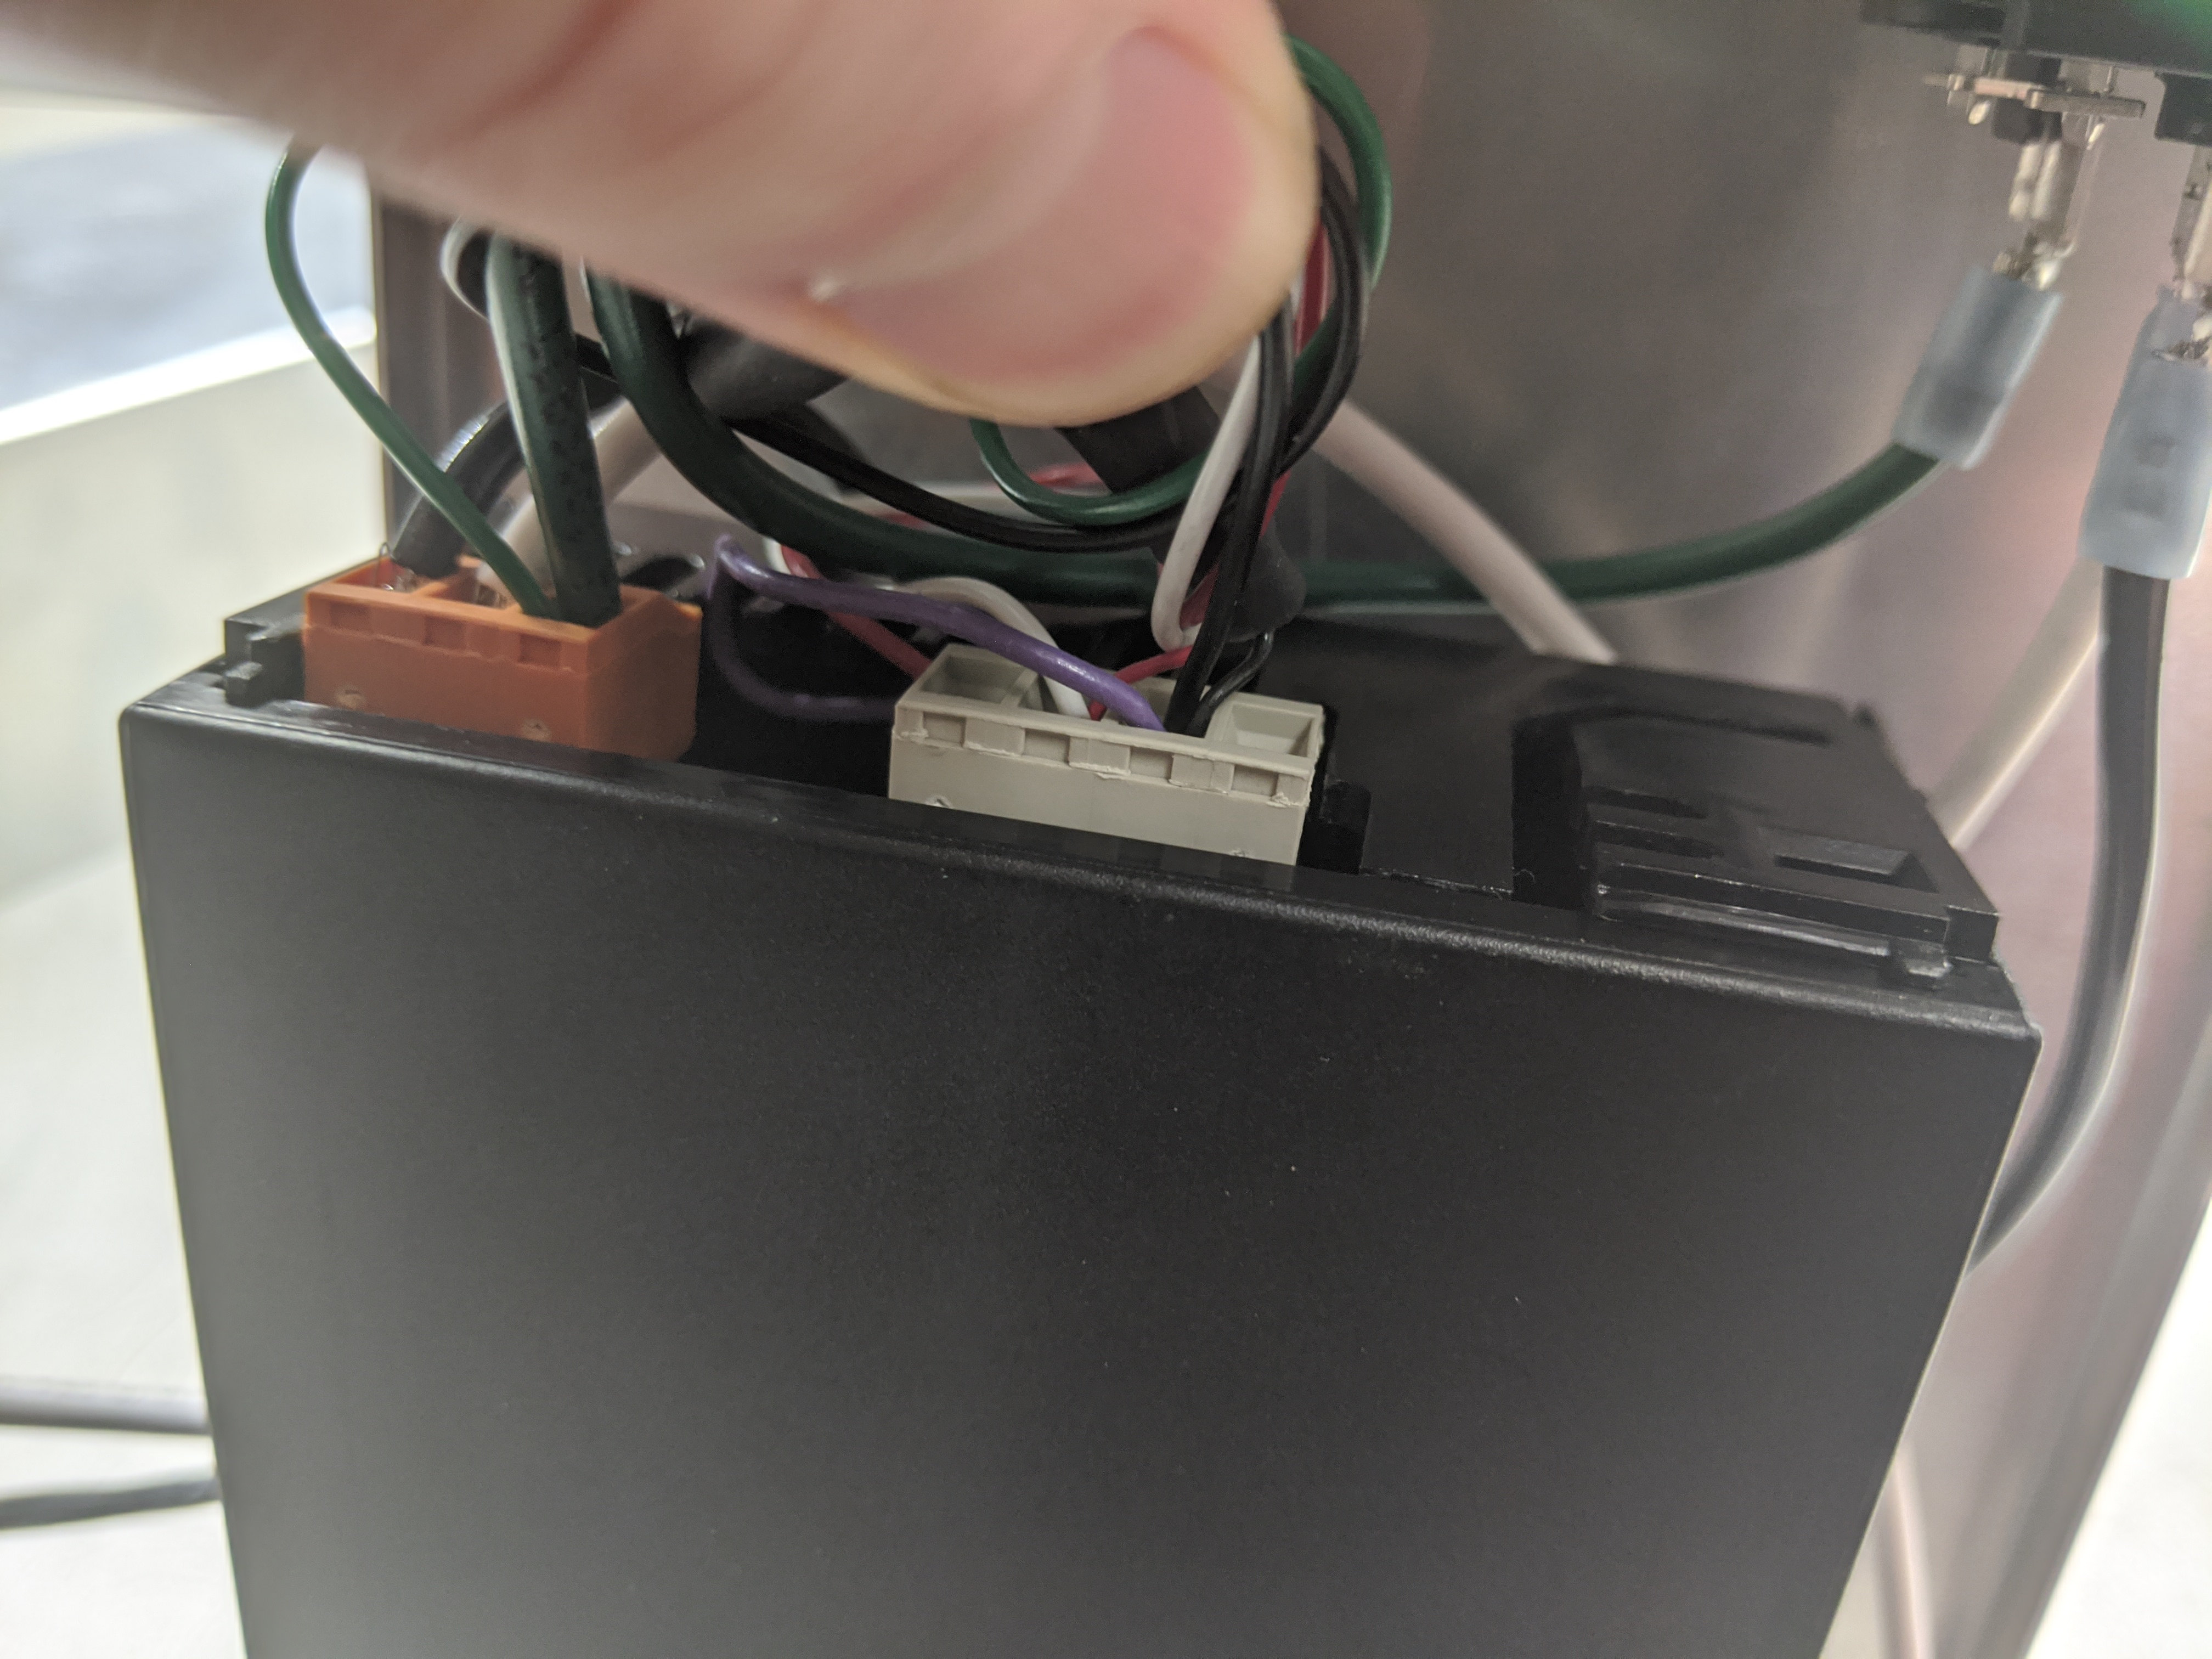
\includegraphics[height=3in]{"./IMG_20200106_153053.jpg"}
\end{frame}

\begin{frame}{Electrocution Hazard}
  \centering
  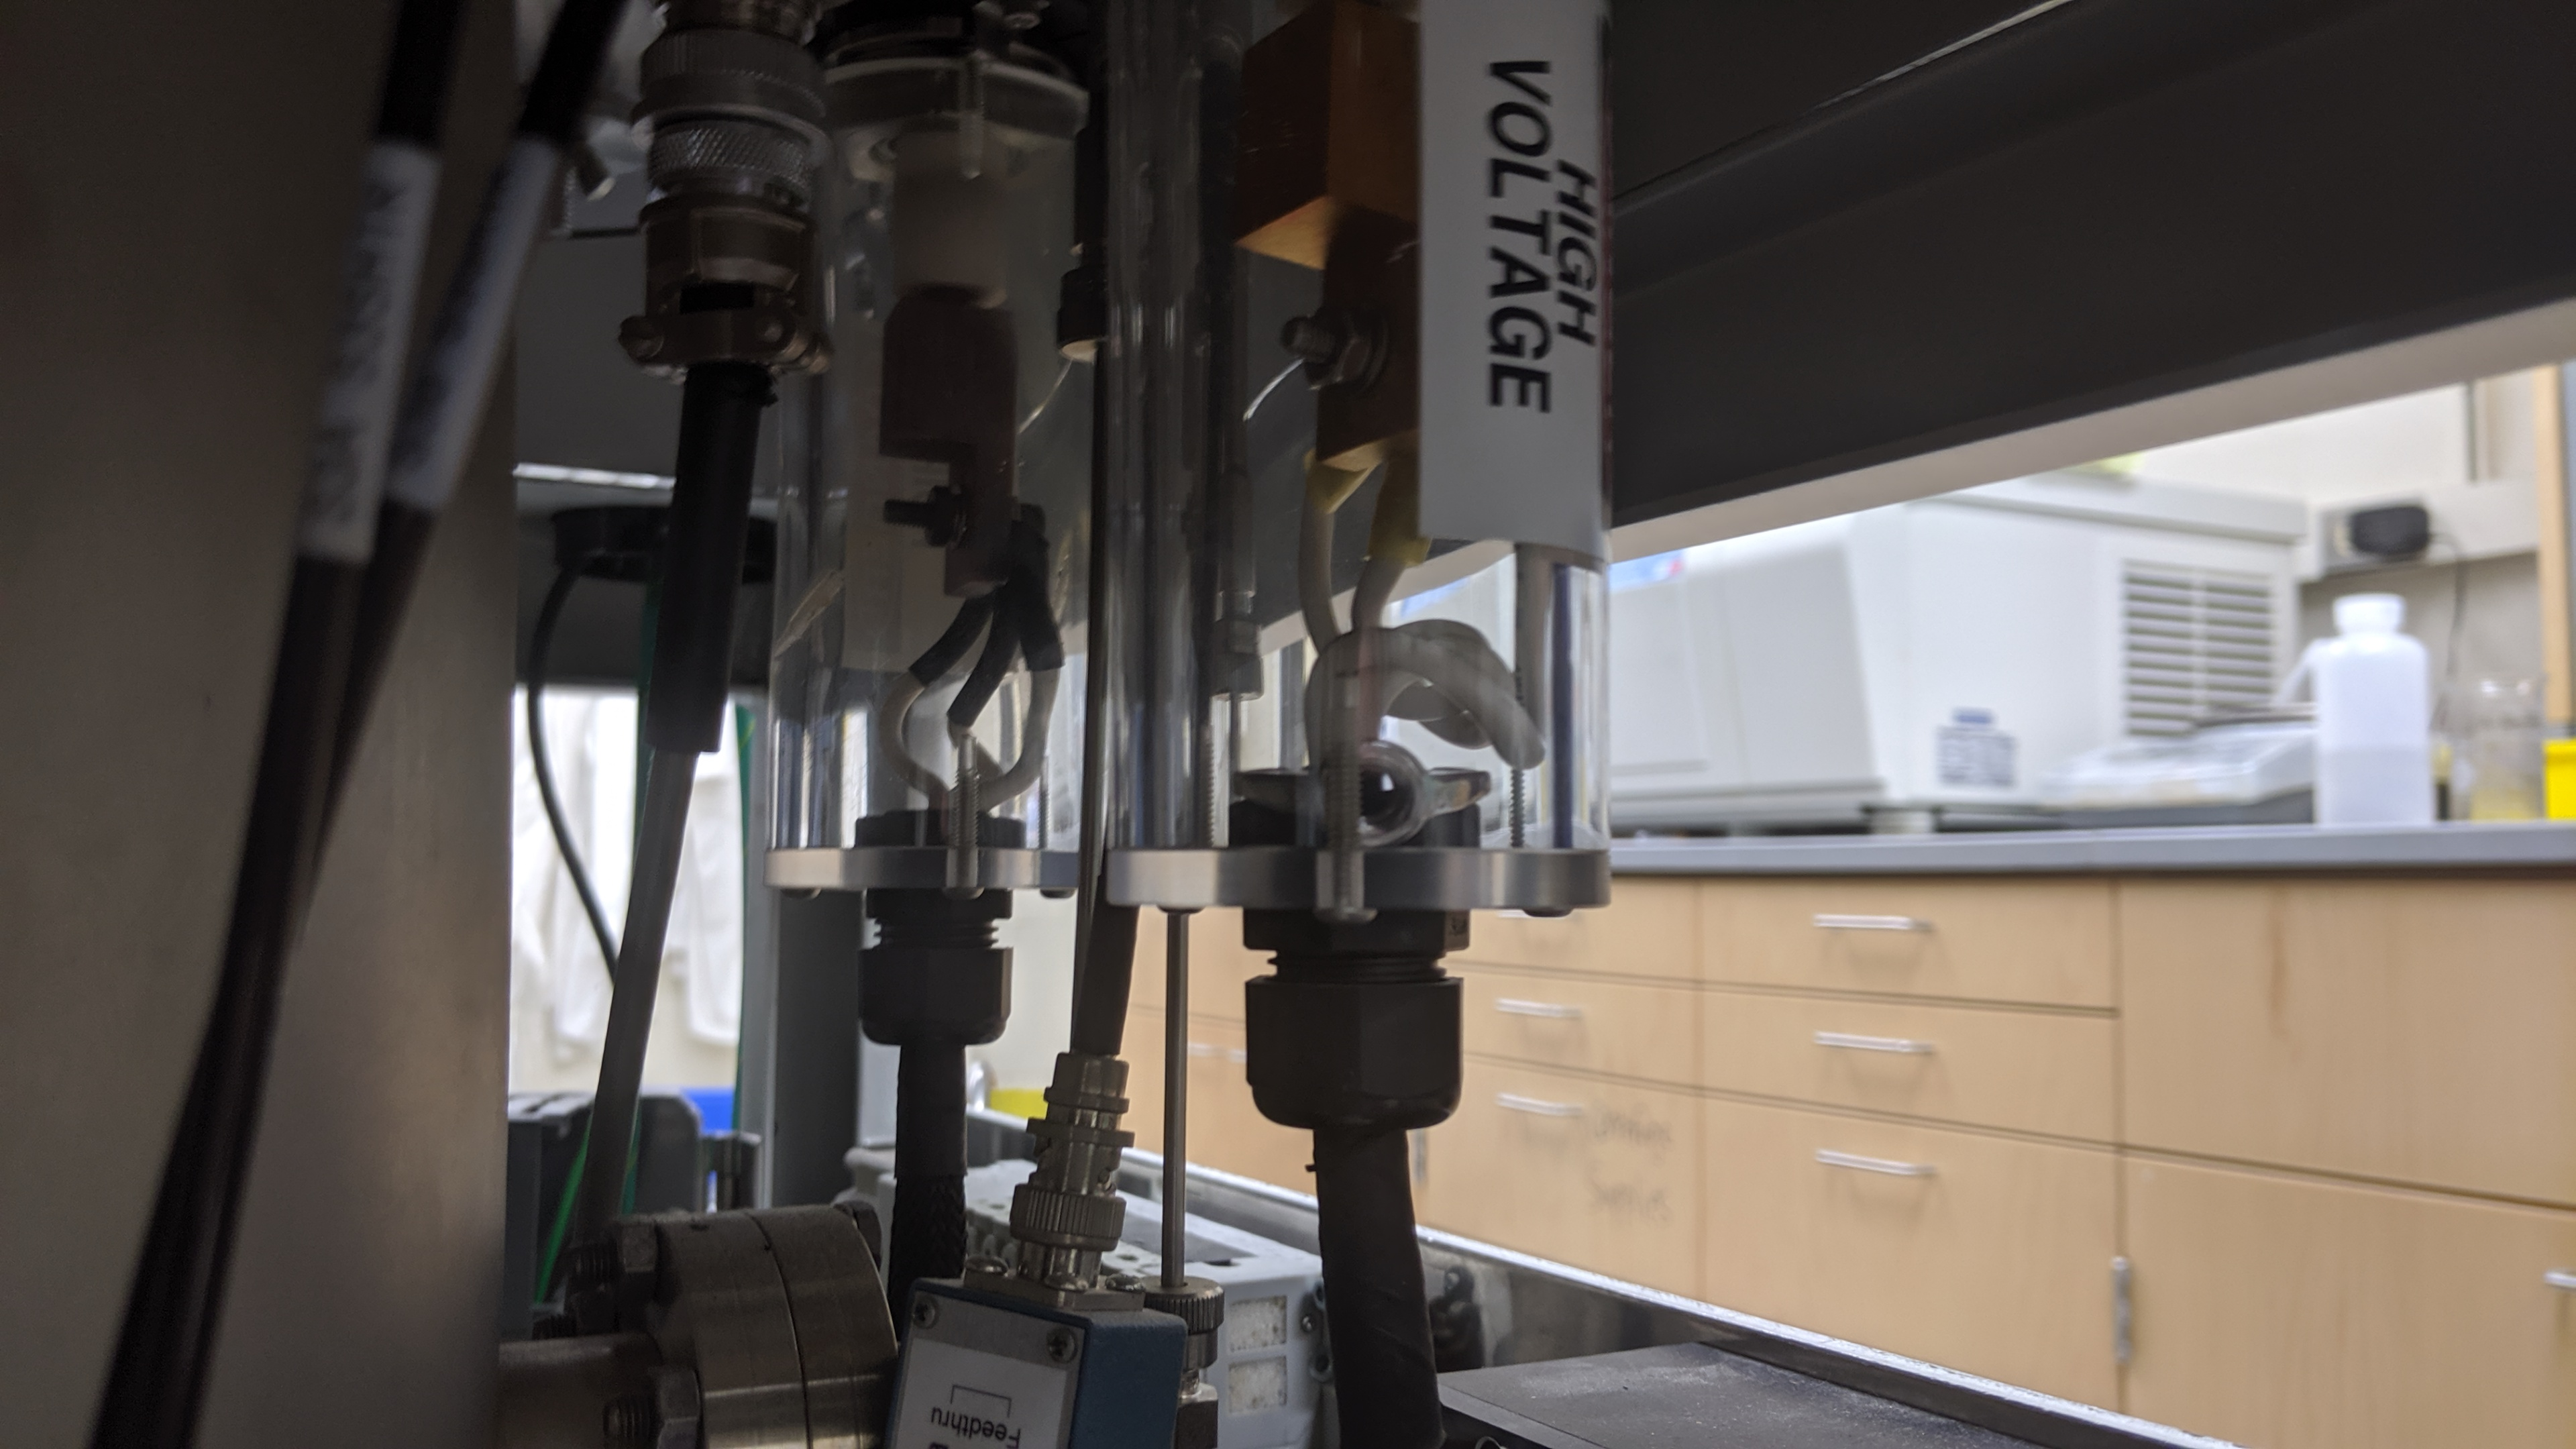
\includegraphics[width=\textwidth]{"./IMG_20191001_140050.jpg"}
\end{frame}

\begin{frame}{Electrocution Hazard}
  \centering
  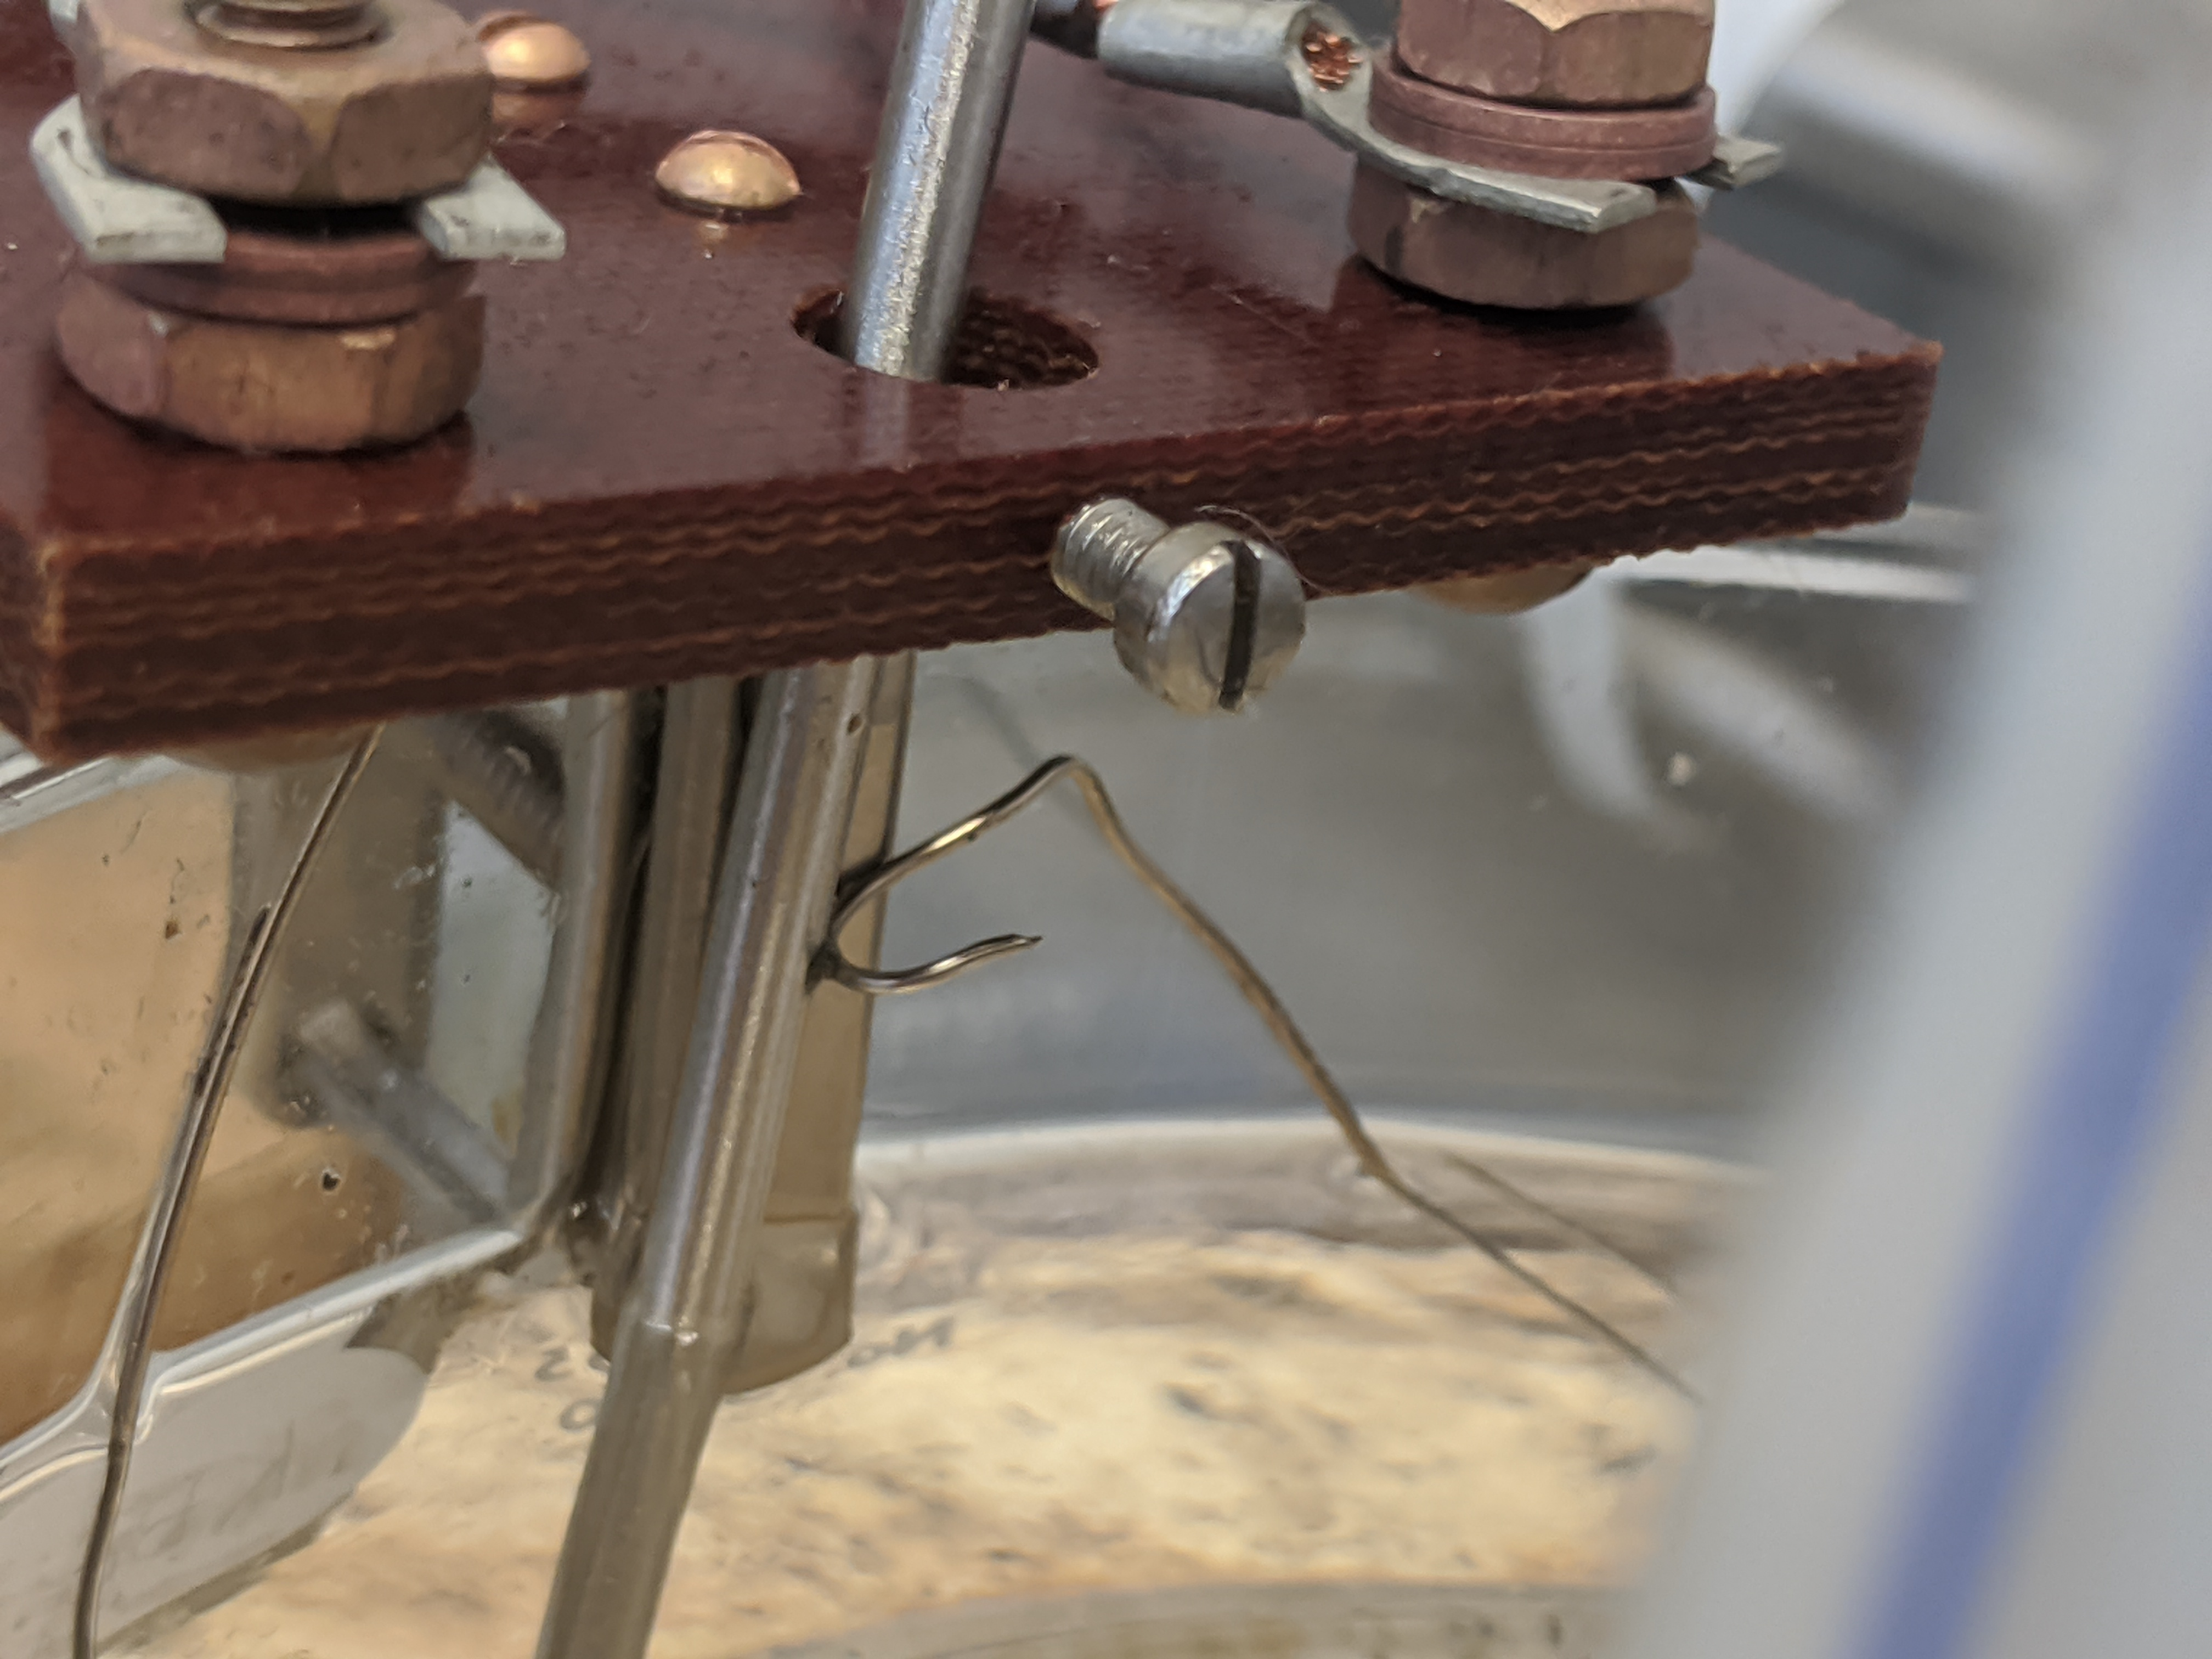
\includegraphics[height=3in]{"./IMG_20200904_131436.jpg"}
\end{frame}

\subsection{Fire}

\begin{frame}{Electrical Fire}
  When an electrical circuit fails it can rapidly cause sparks and get very hot.
  \vfill
  When combined with chemicals, this situation can become explosive.
  \vfill
  Even low voltage circuits are capable of getting very hot. \\
  Power is product of voltage and current.
\end{frame}

\begin{frame}{Recommendations for Avoiding Electrical Fire}
  Ensure that circuits are not overloaded.
  \begin{itemize}
    \item Recognize which devices are drawing a lot of power.
    \begin{itemize}
      \item Heaters, ovens
      \item Pumps
      \item Motors
    \end{itemize}
    \item Be aware which devices share a circuit.
    \item Never use extension cords or power strips.
    \item When in doubt, ask! We can get new power outlets installed into your lab when necessary.
  \end{itemize}
\end{frame}

\begin{frame}{Recommendations for Avoiding Electrical Fire}
  Use good housekeeping.
  \begin{itemize}
    \item Do not crowd multiple appliances into small spaces.
    \item Regularly inspect power cords for damage.
    \item Keep appliances clean, free from chemical buildup.
    \item Dispose of broken appliances quickly.
  \end{itemize}
\end{frame}

\begin{frame}{Recommendations for Avoiding Electrical Fire}
  Protect against catastrophic failure.
  \begin{itemize}
    \item Ensure that devices have fuses and/or breakers.
    \item When designing heating systems, consider incorporating thermal fuses.
    \item Ground exposed metal.
  \end{itemize}
\end{frame}

\begin{frame}{Fire Hazard}
  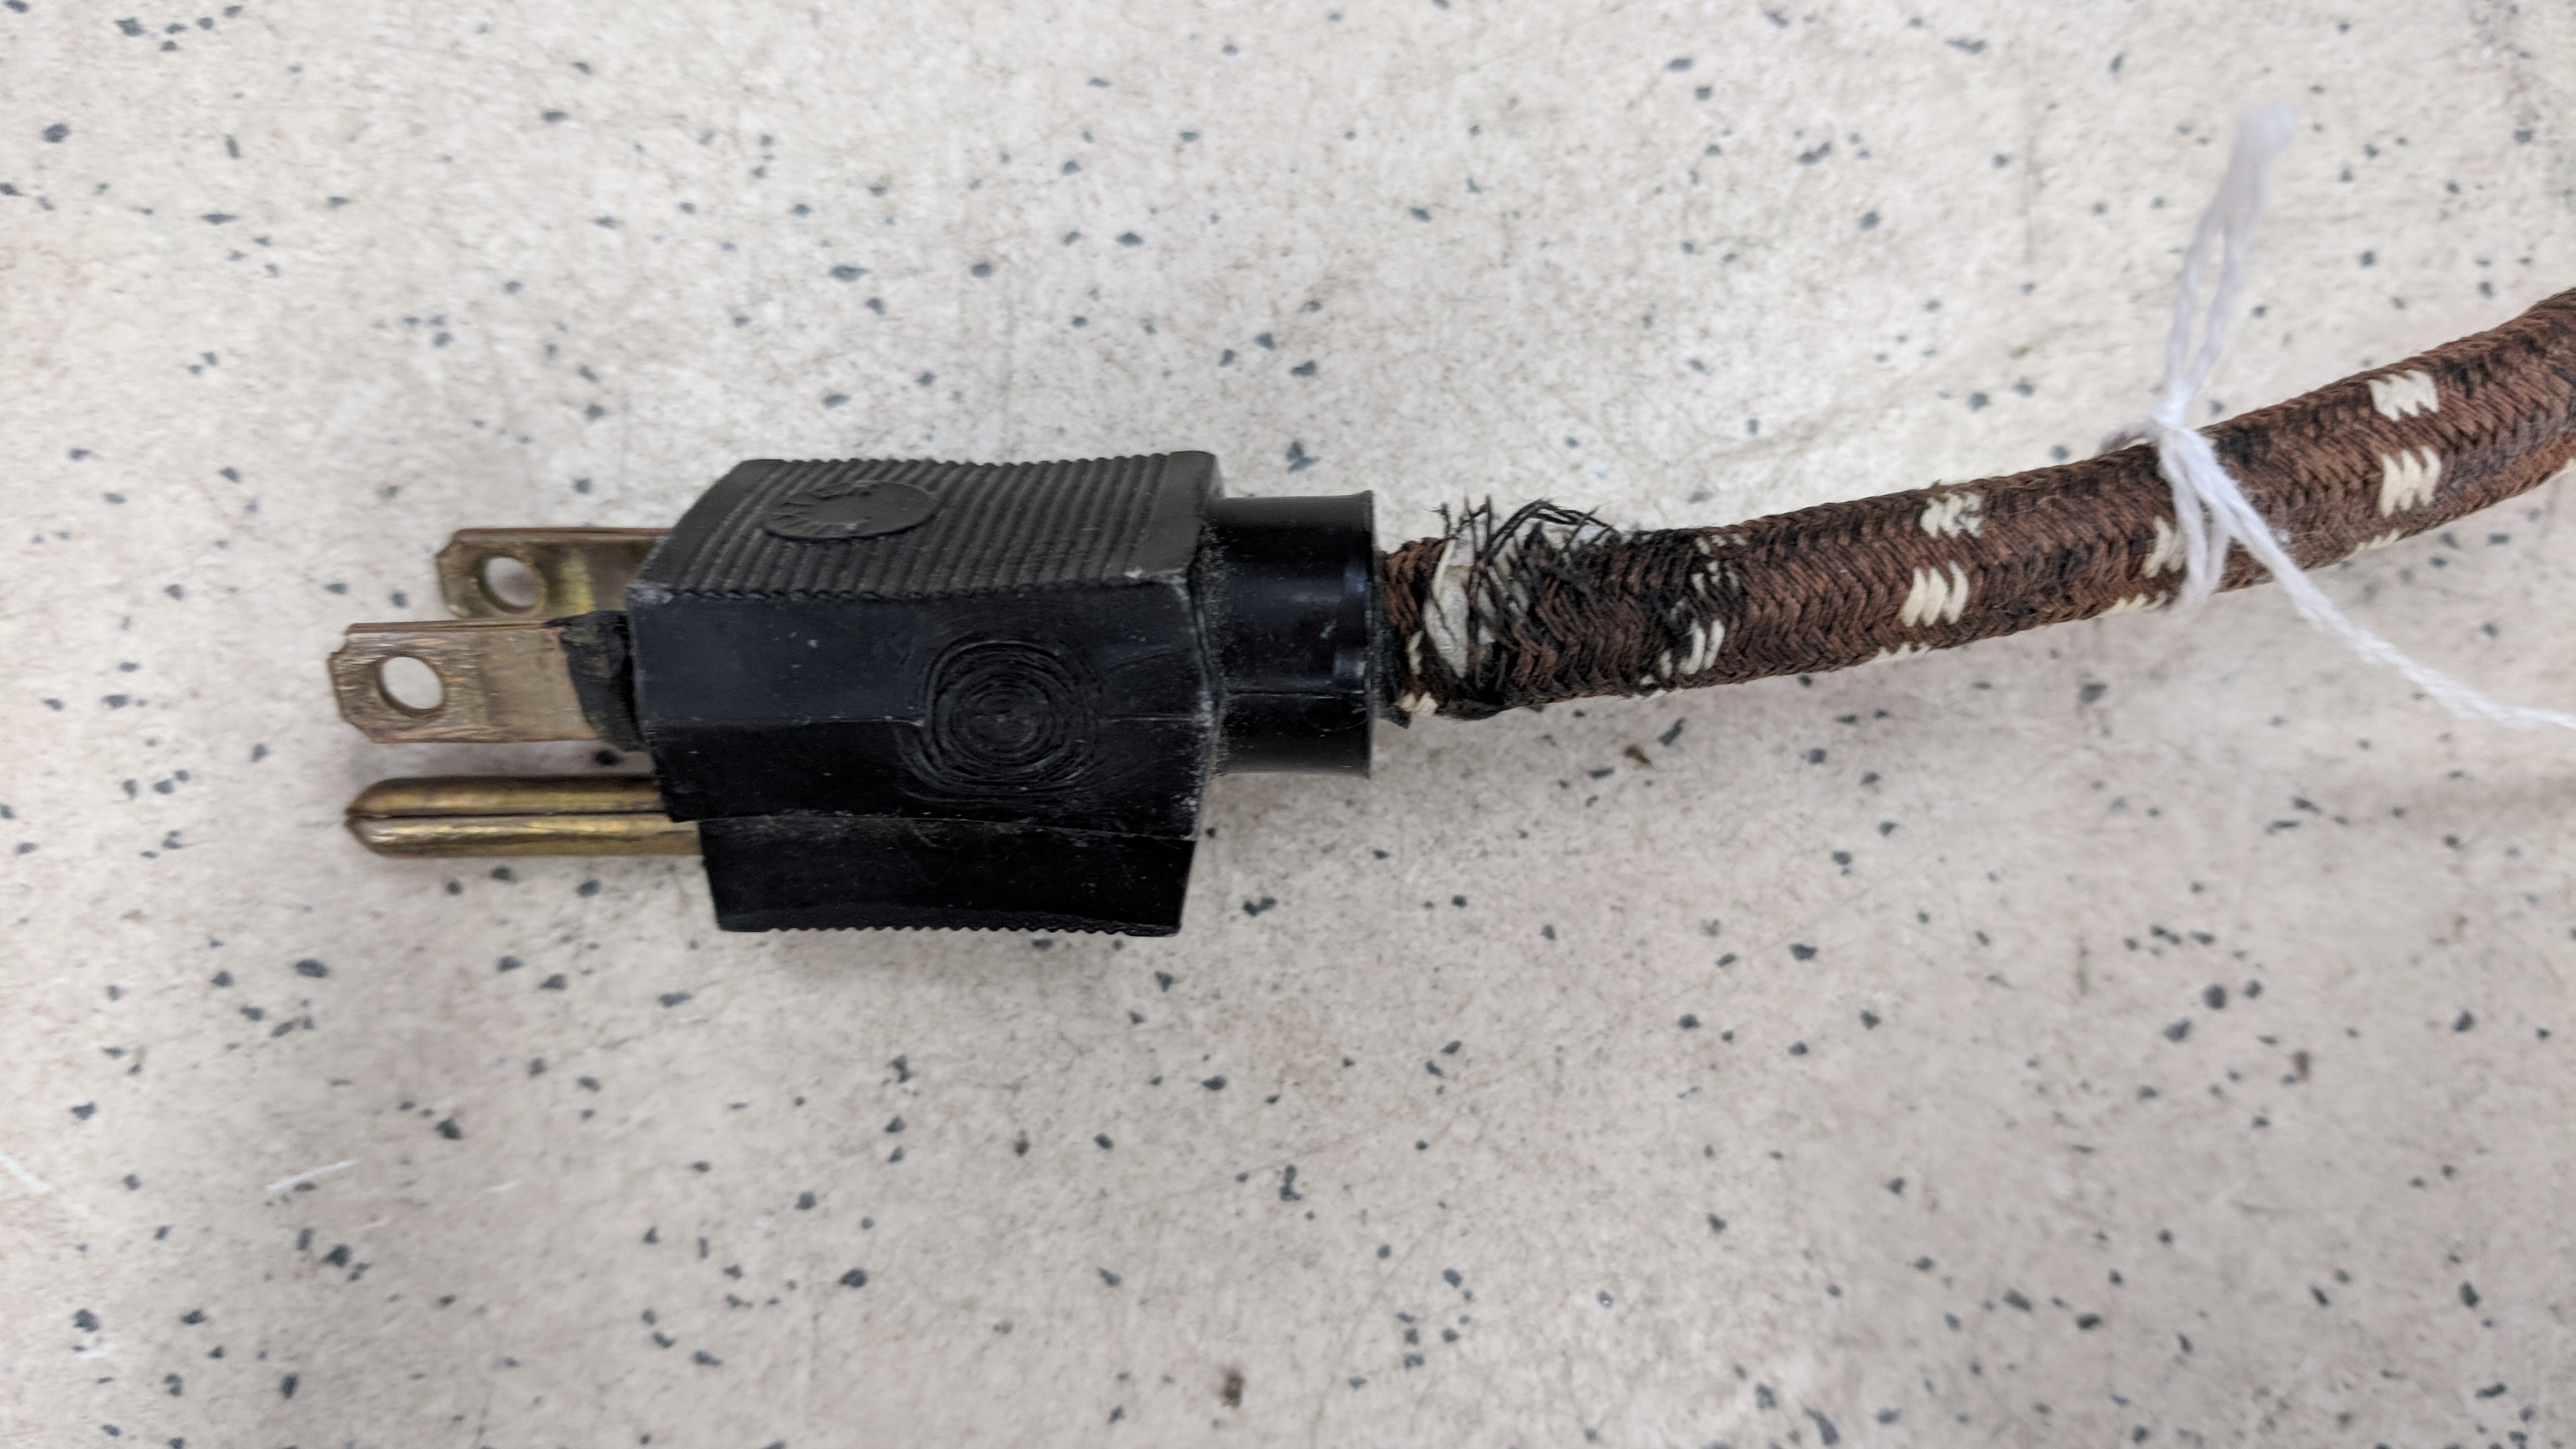
\includegraphics[width=\textwidth]{"./IMG_20181009_153609.jpg"}
\end{frame}

\begin{frame}{Fire Hazard}
  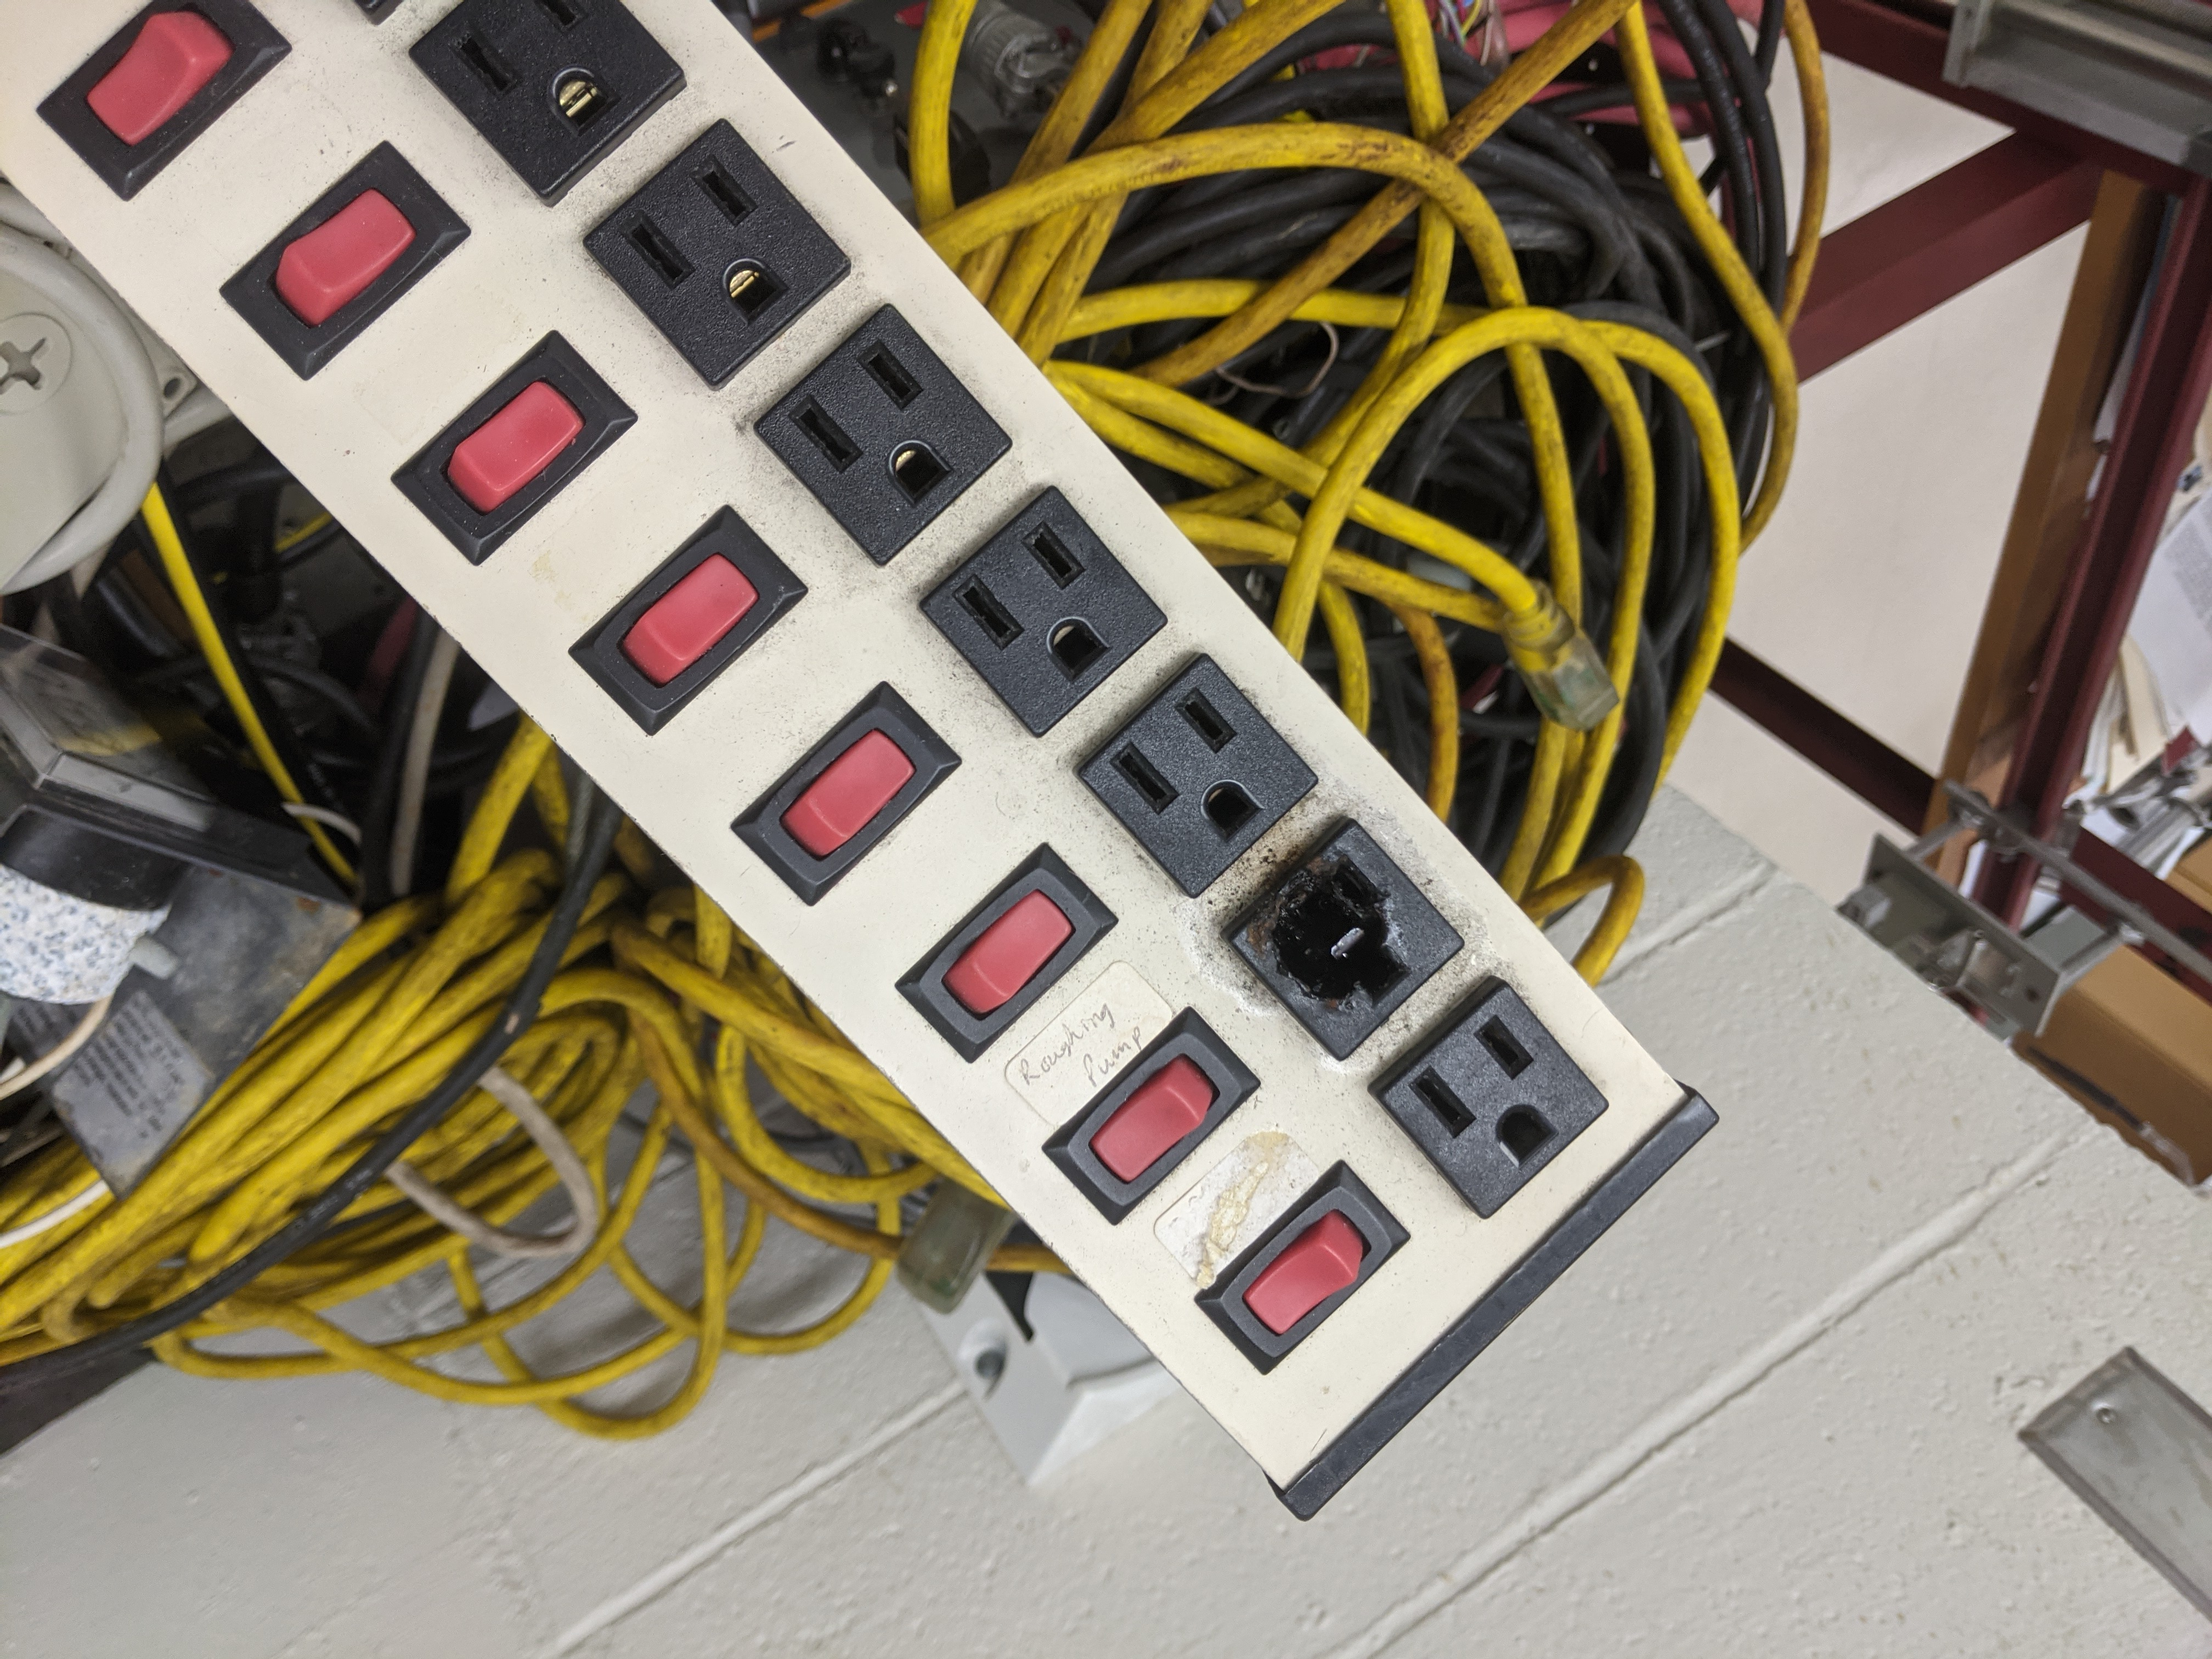
\includegraphics[width=\textwidth]{"./PXL_20201216_221308084.jpg"}
\end{frame}

\begin{frame}{Fire Hazard}
  Grounding, spark hazard.
\end{frame}

\begin{frame}{Cable Ratings}
  \begin{columns}
    \begin{column}{0.33\textwidth}
      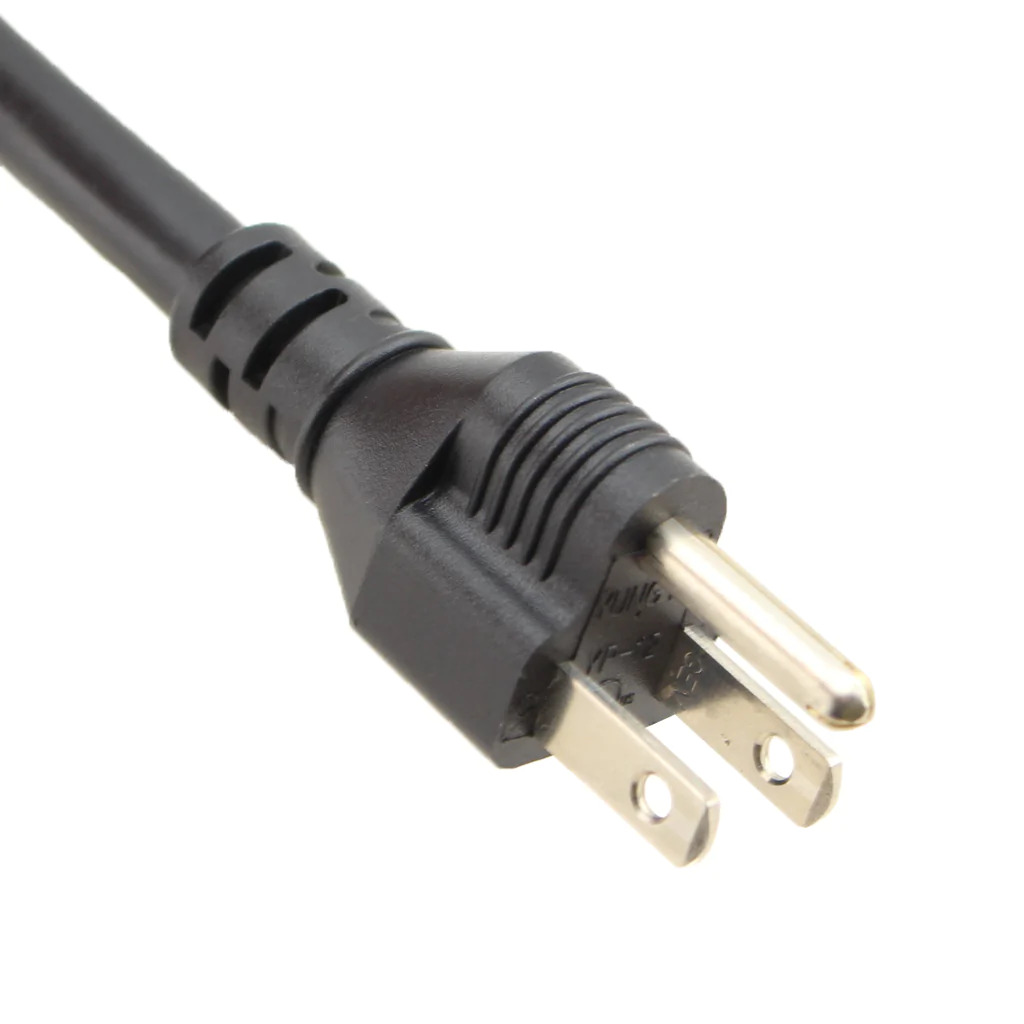
\includegraphics[width=\textwidth]{"./5-15.jpg"}
    \end{column}
    \begin{column}{0.67\textwidth}
      NEMA 5-15
      \\
      120 V
      \\
      Up to 15 amps, but many cables 10 amps!
    \end{column}
  \end{columns}
\end{frame}

\begin{frame}{Cable Ratings}
  \begin{columns}
    \begin{column}{0.33\textwidth}
      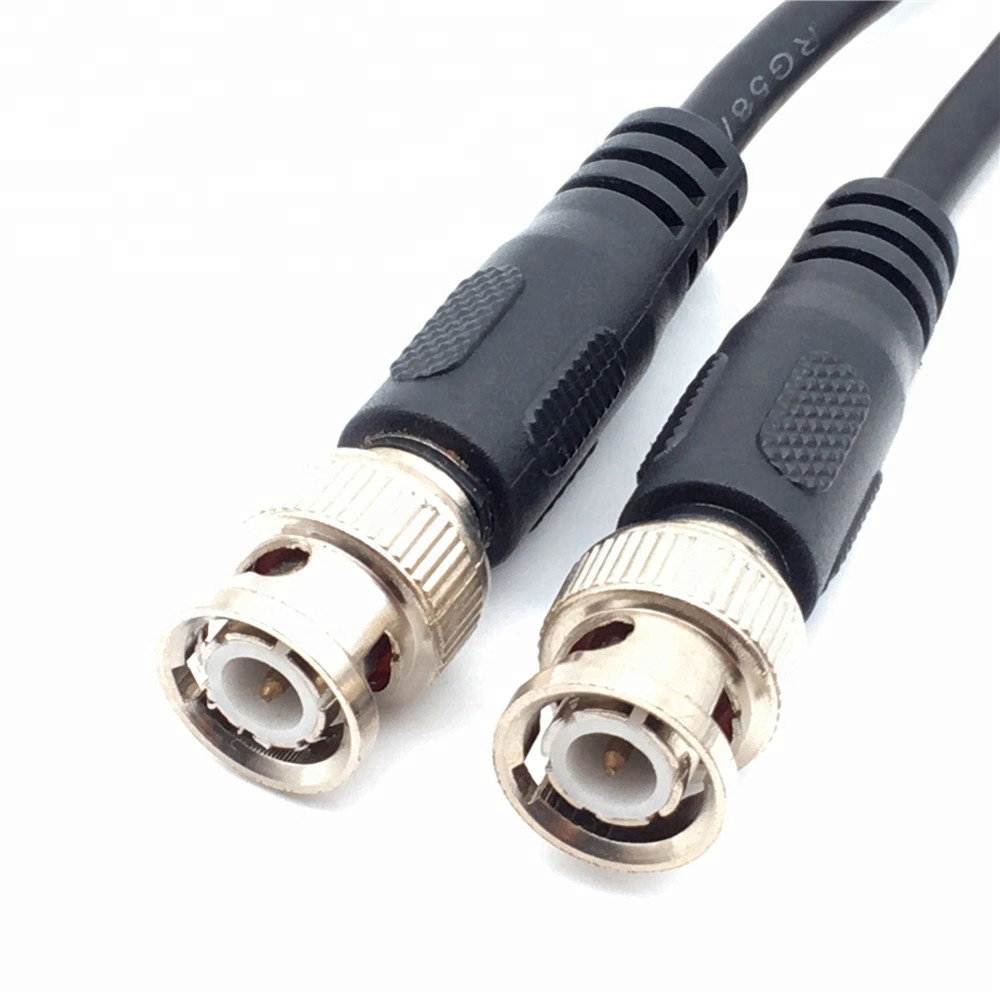
\includegraphics[width=\textwidth]{"./HTB1je_xKXGWBuNjy0Fbq6z4sXXad.jpg"}
    \end{column}
    \begin{column}{0.67\textwidth}
      BNC
      \\
      500 V
      \\
      Typically 1 Amp
      \\
      Use SHV connectors for high voltage (!!!)
    \end{column}
  \end{columns}
\end{frame}

\begin{frame}\frametitle{Other Ideas}
  interlocks
  proper enclosures
  thermal fuse
\end{frame}

\begin{frame}\frametitle{Wiring Mess}
  \centering
  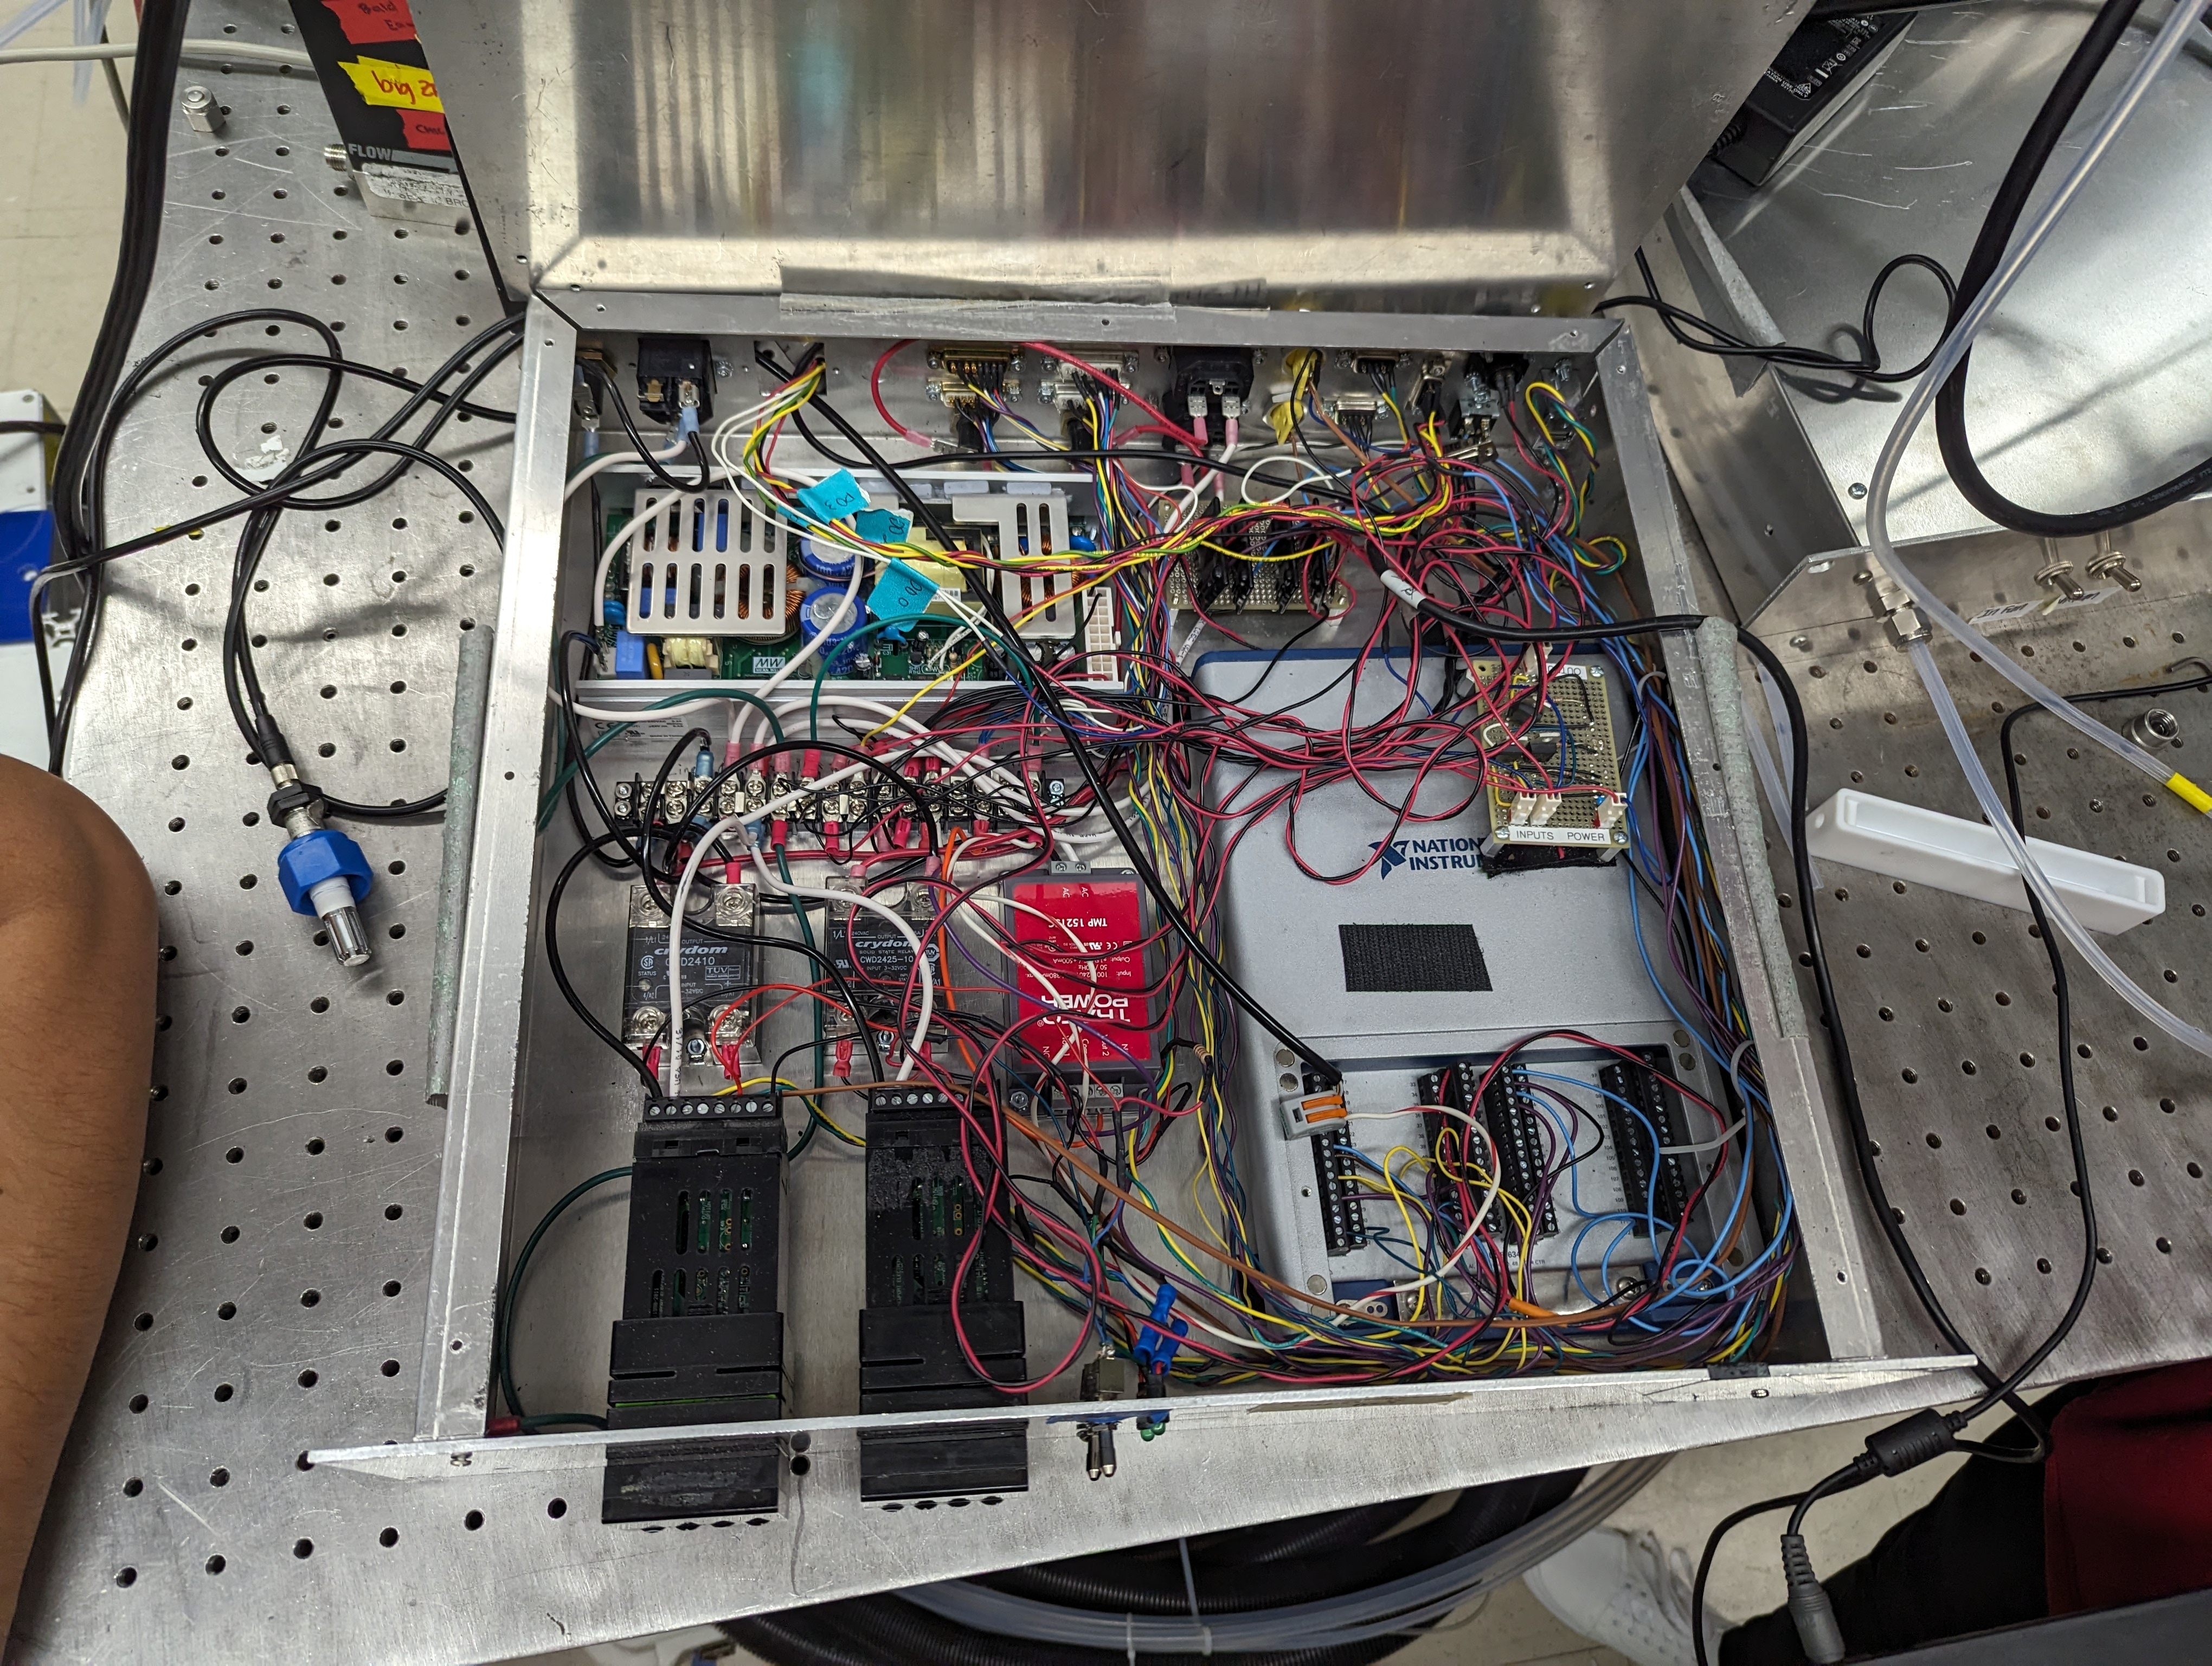
\includegraphics[width=4in]{"./wiring-mess.jpg"}
\end{frame}

\section{Conclusion}

\begin{frame}\frametitle{Conclusion}
  Academic electronics shops contain staff working with researchers to best utilize electronic research equipment.
  \vfill
  Shop staff are professionals who care about electrical safety.
  \vfill
  Your institution might have a research electronics shop---consider reaching out!
\end{frame}

\begin{frame}\frametitle{Thank You}
  \begin{columns}
    \begin{column}{0.33\textwidth}
      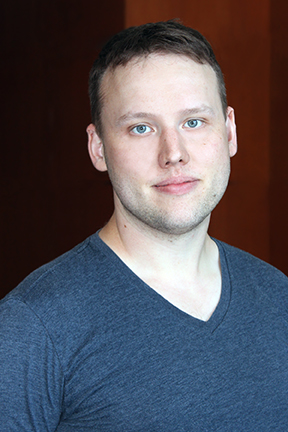
\includegraphics[width=\textwidth]{"./Thompson_Blaise_LowRes.jpg"}
    \end{column}
    \begin{column}{0.67\textwidth}
      Blaise Thompson \\
      Chemistry Electronics Shop \\
      blaise.thompson@wisc.edu
      \vskip 3 em
      Love to learn about research \& electronics.\\
      Let's chat!
      \vskip 3 em
      \hl{Questions?}
    \end{column}
  \end{columns}
\end{frame}

\end{document}
